\chapterimage{Fig/Chapter2/mott_cover_2.png}

\chapter{Optical lattices and the Bose-Hubbard model}

\label{sec:chapter_2}

Quantum gases loaded in optical lattices (lattice gases for short) are one of the paramount examples of Quantum Simulation systems. The periodical trapping potential indeed well reproduces the crystal structure of condensed matter system and allows to study relatively simple Hamiltonians such as the Bose- and Fermi-Hubbard Hamiltonians or the Ising model \cite{bloch2005ultracold} that however account for interactions and show strong correlations effects. The main advantages of this experimental platform is that the different parameters of the Hamiltonians can be set and controlled, while information about the system can be accessed using a variety of experimental techniques as described in the introduction to this manuscript. Following the proposition of \cite{jaksch1998cold}, the experimental observation of the Superfluid to Mott Insulator transition in 2002 \cite{greiner2002quantum} sparked interest in the community and lead to the development of the field from the early 2000s up until this day.

In this chapter, we expose the main elements of the Bose-Hubbard theory of lattice gases and briefly study the Superfluid to Mott insulator transition. We then show how and under which conditions the in-trap momentum distribution of the gas can be accessed through Time-Of-Flight measurements, before drawing the connection with the Bogoliubov theory exposed in Chapter \ref{sec:chapter_1}. The goal of this chapter is to give all the essential points necessary to obtain a system in which the \kmk pairs of the quantum depletion can be experimentally observed, rather than providing a detailled description of Bose-Hubbard physics. For a more thorough study of the superfluid-to-Mott Insulator transition with our experimental apparatus, we refer the reader to the manuscript of Cécile Carcy \cite{carcy_these}.




\section{The Bose-Hubbard Model}

\label{sec:BH_model}

We consider a 3D lattice potential with cubic symmetry and spacing $d$:

\begin{equation}
    V(\bm{r})=V_{0}\left[\sin ^{2}\left(\frac{k_{d}}{2} x\right)+\sin ^{2}\left(\frac{k_{d}}{2} y\right)+\sin ^{2}\left(\frac{k_{d}}{2} z\right)\right] + V_{\mathrm{ext}} (x,y,z)
\end{equation}

\noindent where $k_d=\frac{2 \pi}{d}$ is the associated wave-vector and $V_0$ the lattice depth. For convenience, $V_0$ is usually expressed in units of recoil energy $V_0 = s E_{\rm{r}}$ with $E_r=h^2/ 8 m d^2$. In most experiments, such a potential is created with countra-propagating pairs of Gaussian laser beams. The term $V_{\mathrm{ext}} (x,y,z)$ denotes the additional harmonic potential that results from the Gaussian shape of the beams. For simplicity of calculations, we will first treat here the homogeneous case $V_{\mathrm{ext}} (x,y,z)=0$.

We consider an ensemble of $N$ bosons that interact with one another with the potential $U_{\rm{int}} ( \bm{r}_1, \bm{r}_2)$ loaded in the lattice potential $V(\bm{r})$. The Hamiltonian of the system writes:

\begin{equation}
    \hat{H}=\sum_{i=1}^{N} \frac{\bm{p}_{i}^{2}}{2 m}+\sum_{i=1}^{N} V\left(\bm{r}_{i}\right) + \sum_{i}^{N} \sum_{j>i}^{N} U_{\text{int}}\left(\bm{r}_{i}, \bm{r}_{j}\right)
    \label{eq:H_lattice_full}
\end{equation}

\subsubsection{Non-interacting lattice gas}

To begin with, we consider that the atoms are non-interacting and study the simplified Hamiltonian:

\begin{equation}
    \hat{H}_0=\sum_{i=1}^{N} \frac{\bm{p}_{i}^{2}}{2 m}+\sum_{i=1}^{N} V\left(\bm{r}_{i}\right)
\end{equation}

\noindent As the Hamiltonian is separable along the 3 directions of space and the gas of atoms is non-interacting, we can simply work with the one-dimensional, single particle Hamiltonian:

\begin{equation}
    \hat{H}_{\rm{1D}} = \frac{p_x^2}{2m} + \sin^2 \Big(\frac{k_d}{2} x \Big)
\end{equation}

\noindent To find the eigenstates of this Hamiltonian, we use the Bloch's theorem \cite{ashcroft1976solid}:

\begin{tcolorbox}[colback=red!5!white,colframe=red!75!black,title=\textbf{Bloch's theorem}]
\label{sec:bloch}
The eigenstates of a Hamiltonian corresponding to a spatially periodic potential $V(\bm{r})$ on a lattice $\mathcal{B}$ are Bloch waves $\psi_{\bm{q}}(\bm{r})$, product of a plane-wave $e^{i \bm{r}.\bm{q}}$ and a periodical function on $\mathcal{B}$, $u_{\bm{q}} (\bm{r})$.
\end{tcolorbox}

We therefore look for eigenstates of the form:

\begin{equation}
    \psi_{n,q} (x)= e^{iqx} u_{n,q} (x)
    \label{eq:bloch_wave}
\end{equation}

\noindent with $n \in \N$ and $q \in \R$ the \textbf{quasi-impulsion}. In order to determine the functions $u_{n,q} (x)$ and the energy $E_n (q)$, we inject equation \ref{eq:bloch_wave} in the eigenvalue equation to find that they must verify:

\begin{equation}
    \left[\frac{\left(p_{x}+\hbar q\right)^{2}}{2 m}+V_{0} \sin ^{2}\left(\frac{k_{d}}{2} x\right)\right] u_{n, q}(x)=E_{n}(q) u_{n, q}(x)
\end{equation}

\noindent As $E_n (q)$ is periodic $E_n (q+k_d)= E_n(q) \ \forall (n,q)$, we can restric the definition interval of $q$ to $[-k_d/2, k_d/2]$ which is called the \textbf{first Brillouin zone}. This equation can be easily numerically solved to obtain $u_{n, q}(x)$ and $E_n (q)$. We plot on Fig.-\ref{fig:bloch_bands} the first five energy bands as a function of $q$ in the first Brillouin zone for various values of the lattice amplitude $V_0$. Interestingly, we see that a gap appears between the different bands as we increase $V_0$. For a 3D lattice, the total energy is the sum of the energies along each direction of the lattice. The first excited band then corresponds to two 1D lowest energy bands and one 1D excited band. In order for the gap to appear, the lattice amplitude must be above $V_0 \simeq 2.2 \ E_{\mathrm{r}}$, whereas it is present at all values of $V_0$ in the 1D case.

\begin{figure}
    \centering
    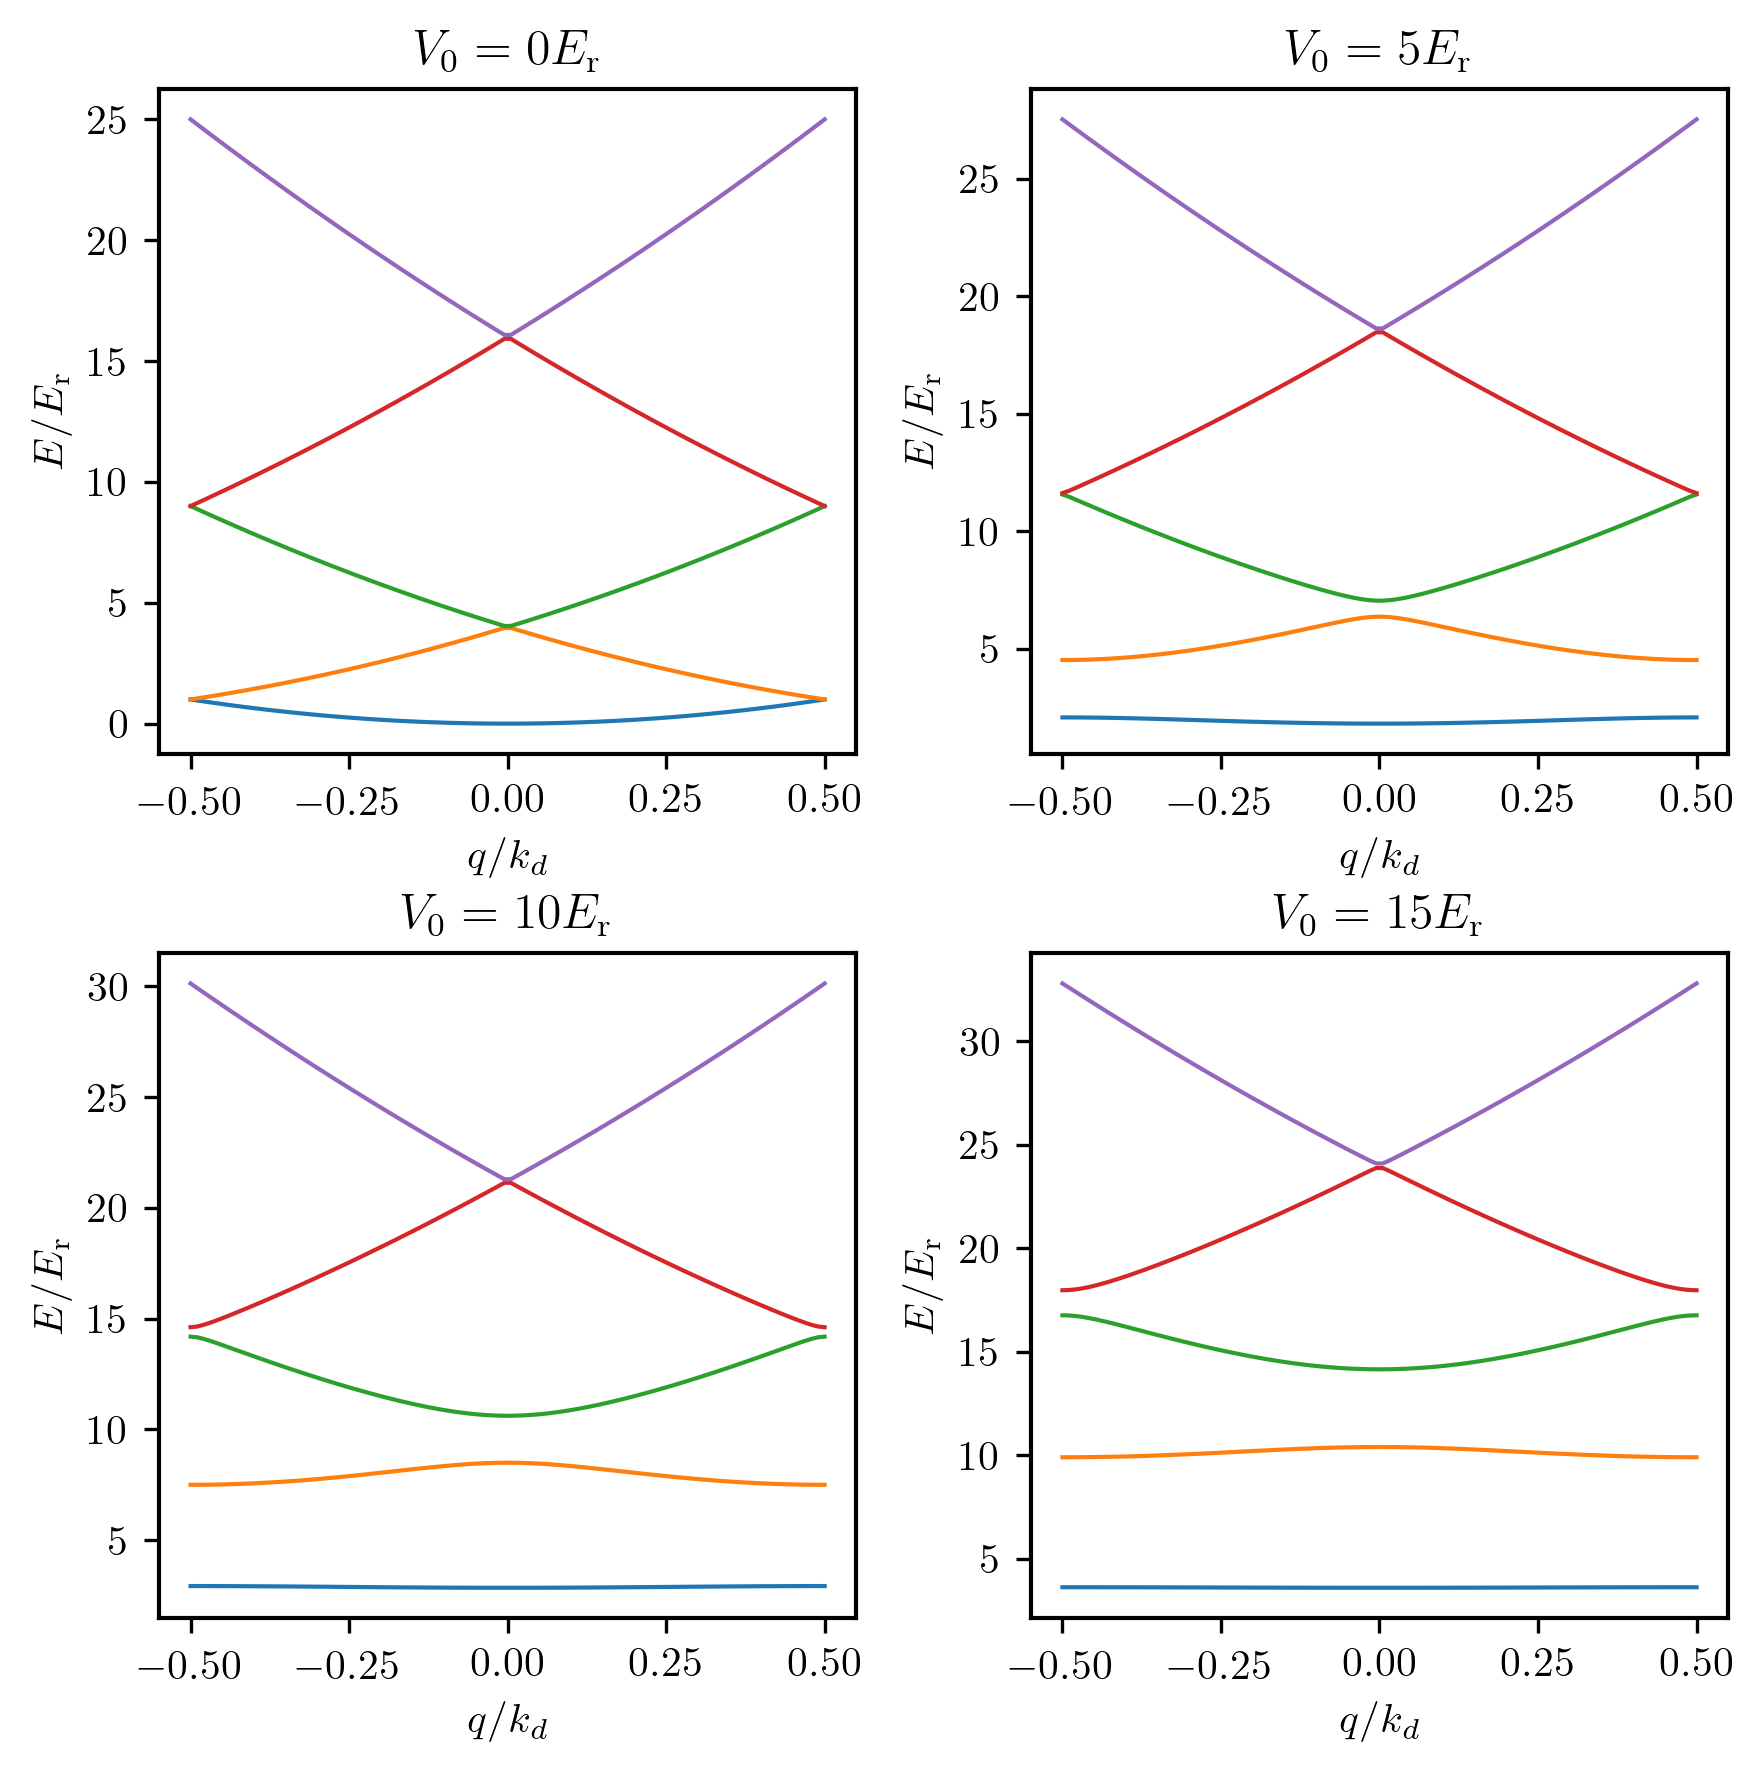
\includegraphics[width=\textwidth]{Fig/Chapter2/bloch_bands.png}
    \caption[First five Bloch energy bands for various lattice amplitudes $V_0$]{First five Bloch energy bands for various lattice amplitudes $V_0$. The gap between the first bands increases as $V_0$ increases.}
    \label{fig:bloch_bands}
\end{figure}

In addition to the Bloch waves, it is possible to define a new kind of functions called the\textbf{ Wannier functions} \cite{wannier1937structure} that are localized near the lattice sites. They are defined from the Bloch waves by:

\begin{equation}
    w_{n, j}(x)=\sqrt{\frac{d}{2 \pi}} \int_{\mathrm{BZ}} \psi_{n, q}(x) e^{-i j q d} \mathrm{~d} q, \quad j \in \mathbb{Z}
    \label{eq:wannier_functions}
\end{equation}

\noindent with BZ denoting an integration over the first Brillouin zone and where $j$ can be interpreted as the index of a lattice site. Actually, we have from equation \ref{eq:wannier_functions} the simple relation:

\begin{equation}
    w_{n, 0}(x-j d)=w_{n, j}(x)
\end{equation}

The Bloch waves can then be re-written with the definition of the Wannier functions and write:

\begin{equation}
    \psi_{n, q}(x)=\left(\frac{d}{2 \pi}\right)^{1 / 2} \sum_{j} w_{n, j}(x) e^{-i j d q}
    \label{eq:bloch_as_wannier}
\end{equation}


\begin{figure}
    \centering
    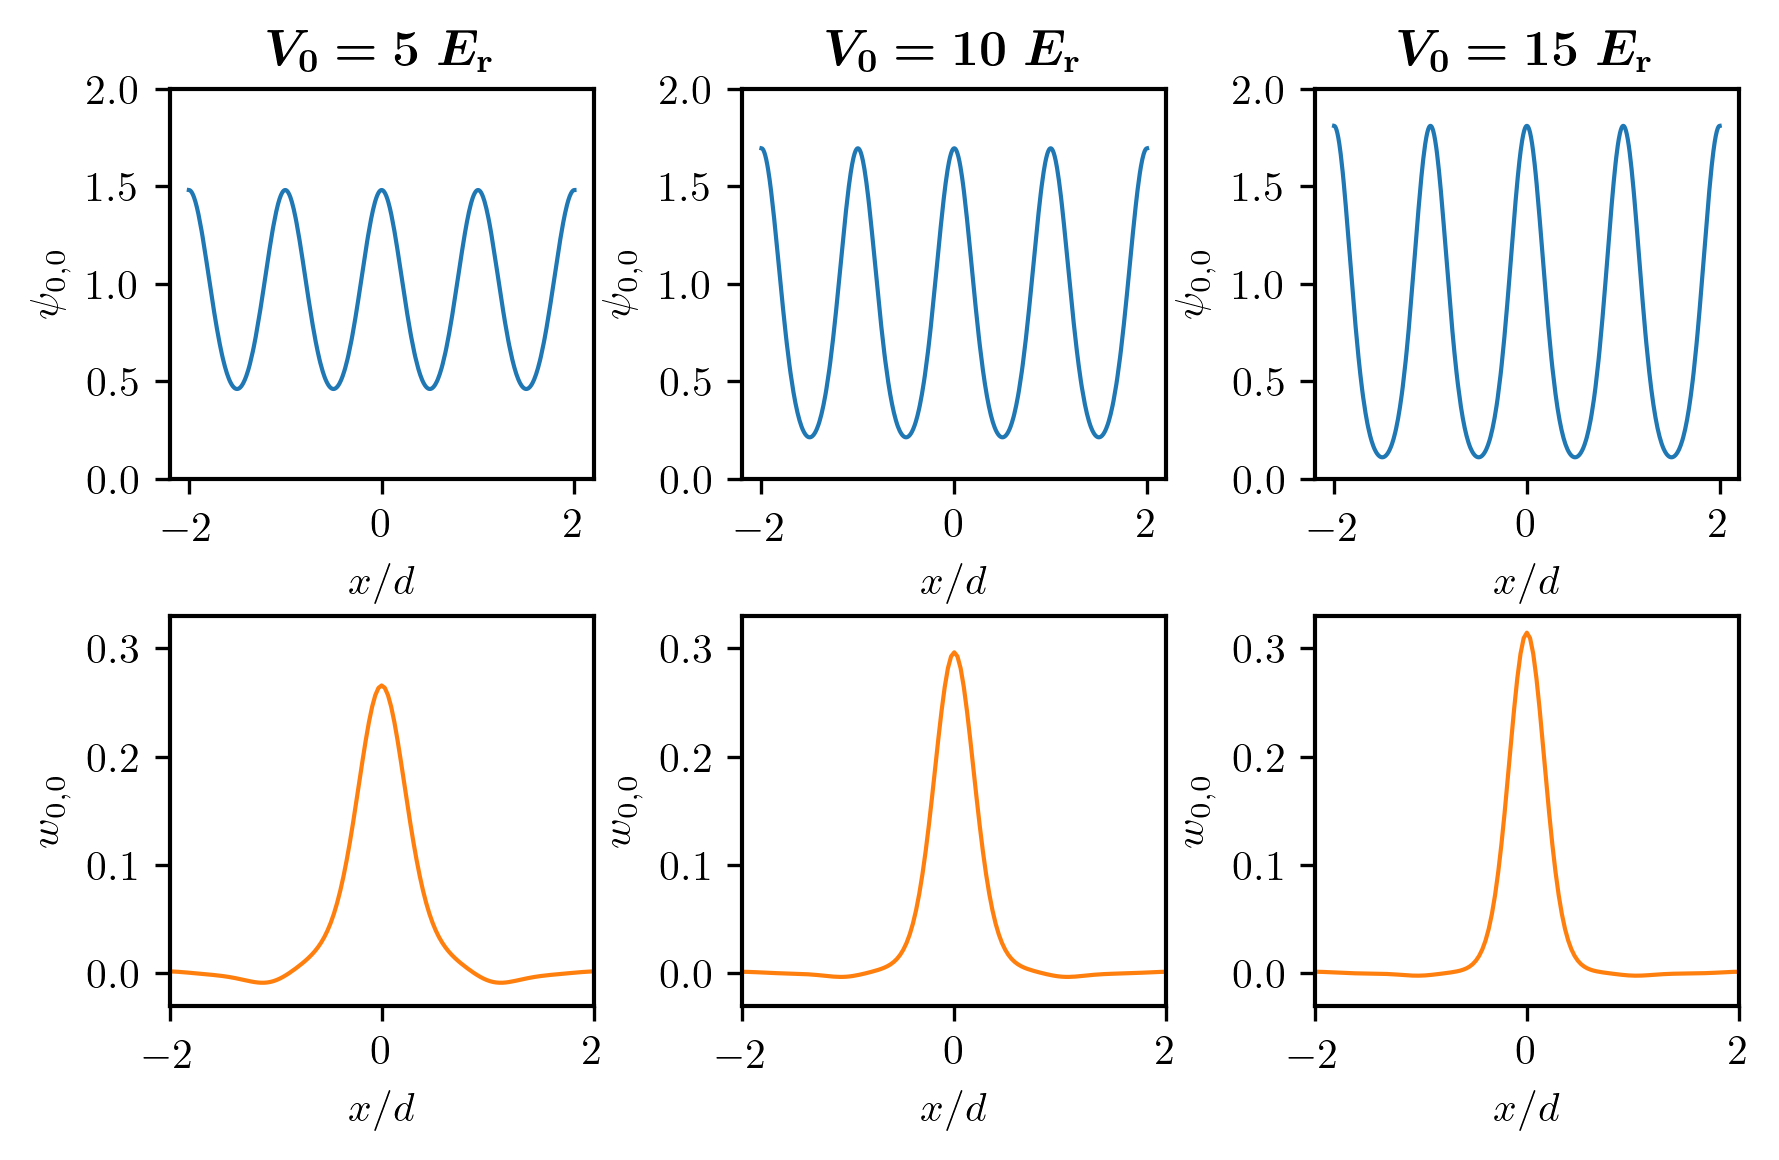
\includegraphics[width=1.05\textwidth]{Fig/Chapter2/bloch_wannier.png}
    \caption[Real parts of the Bloch and Wannier functions for various lattice depths]{Real parts of the Bloch and Wannier functions for various lattice depths. When the lattice depth increases, the Bloch function is increasingly peaked around the lattice sites and the Wannier function gets narrower.}
    \label{fig:bloch_wannier}
\end{figure}

\noindent The Bloch waves are the sum of the localized Wannier function $w_{n, j}$ that can be interpreted as the wave-function of a particle located in lattice site $j$. The Bloch and Wannier functions for various lattice depths are represented on Fig.-\ref{fig:bloch_wannier}.

We can now re-write the Hamiltonian of the system with the newly introduced Wannier functions. To do so, we start by writing it in the Bloch waves basis with the second quantification formalism, introducing the operator $\hat{c}_{n,q}$ that destroys a particle in the Bloch wave $\psi_{n,q}$.

\begin{equation}
    \hat{H}_{\rm{1D}}=\sum_{n} \int_{\mathrm{BZ}} E_{n}(q) \hat{c}_{n, q}^{\dagger} \hat{c}_{n, q} \mathrm{~d} q
    \label{eq:H_bloch}
\end{equation}

\noindent To change into the Wannier function basis as defined in \ref{eq:bloch_as_wannier}, we introduce the operator $\hat{b}_{n,j}$ destroying a particle in the Wannier function $w_{n,j}$ and defined such as:

\begin{equation}
    \hat{c}_{n}(q)=\sqrt{\frac{d}{2 \pi}} \sum_{j} \hat{b}_{n, j} e^{i j d q}
    \label{eq:a_wannier}
\end{equation}

\noindent Injecting equation \ref{eq:a_wannier} in equation \ref{eq:H_bloch}, we get:

\begin{equation}
    \hat{H}_{\rm{1D}}=\sum_{n} \sum_{j, j^{\prime}} J_{n}\left(j-j^{\prime}\right) \hat{b}_{n, j^{\prime}}^{\dagger} \hat{b}_{n,j}
    \label{eq:H_Jn}
\end{equation}

\noindent This Hamiltonian has a nice physical meaning: it describes the tunneling process by which a particle in site $j$ can ``hop'' to another lattice site $j'$ with the tunneling amplitude $J_n (j-j')$ that writes:

\begin{equation}
    J_{n}\left(j-j^{\prime}\right)=\frac{d}{2 \pi} \int_{\rm{BZ}} e^{i\left(j-j^{\prime}\right) q d} E_{n}(q) \mathrm{d} q
\end{equation}

\noindent This expression tells that the probability for a particle to tunnel from lattice site $j$ to $j'$ is reduced as the distance between the two sites $j$ and $j'$ increases and as the potential barrier, \ie the lattice depth, increases.

As for the rest of this thesis, we will focus on the ground-state properties of the system and therefore assume that the lowest energy band is the only one populated. This assumption is valid as long as $V_0 \geq 2.2 \ E_{\rm{r}}$ at which the gap is opening and the typical excitation energy $\Delta E$ is smaller than the gap $\Delta=E_1-E_0$. In addition, for $V_0 \geq 5 \ E_{\rm{r}}$ \cite{gerbier_notes}, we can use the tight-binding approximation for which only the tunneling events between adjacent sites are non-negligible. We thus simplify the Hamiltonian \ref{eq:H_Jn} by replacing  $J_{n}\left(j-j^{\prime}\right)$ by a constant $J$ denoting the probability to tunnel between adjacent lattice sites, 

\begin{equation}
    J=-J_0(1)
\end{equation}

\noindent so that $J$ is positive. Finally, we obtain the first term of the Bose-Hubbard Hamiltonian:

\begin{equation}
    \hat{H}_{\rm{1D}} = -J \sum_{\mean{i,j}} \hat{b}^{\dagger}_i \hat{b}_j
    \label{eq:H_band}
\end{equation}

\noindent where $\mean{i,j}$ denotes the ensemble of all adjacent lattice sites $i$ and $j$. In the 3D case, the expression of the Hamiltonian remains the same.

\subsubsection{Interaction term}
We now turn to studying the interaction term that we had left out in the full Hamiltonian of equation \ref{eq:H_lattice_full}. In the formalism of second quantification, the short-range, $s$-wave, 1D interaction Hamiltonian writes:

\begin{equation}
    \hat{H}_{\mathrm{int}}=\frac{1}{2} \int d x \int d x' U_{\mathrm{int}}\left(x, x'\right) \hat{\Psi}^{\dagger}(x) \hat{\Psi}^{\dagger}\left(x'\right) \hat{\Psi}\left(x^{\prime}\right) \hat{\Psi}(x)
\end{equation}

\noindent with $\hat{\Psi}(x)$ the operator destroying a particle at position $x$ that we write in terms of Wannier functions as:

\begin{equation}
    \hat{\Psi}(x)=\sum_{j} w_{j}(x) \hat{b}_{j} = \sum_{j} w_{0}(x-x_j) \hat{b}_{j} 
    \label{eq:atom_operator_lattice}
\end{equation}

\noindent Note that we dropped the energy band number $n$ as we are considering only the lowest energy band. We approximate the interactions to be contact, repulsive interactions so that:

\begin{equation}
    U_{\rm{int}}= g \delta (x_1 - x_2)
\end{equation}

\noindent with $g=\dfrac{4 \pi \hbar^2 a_s}{m}$ the strength of the interactions. The interaction Hamiltonian can then be re-written:

\begin{equation}
    \hat{H}_{\mathrm{int}}=\frac{g}{2} \sum_{j_{1}} \sum_{j_{2}} \sum_{j_{3}} \sum_{j_{4}} \hat{b}_{j_{4}}^{\dagger} \hat{b}_{j_{3}}^{\dagger} \hat{b}_{j_{2}} \hat{b}_{j_{1}} \int w_{j_{4}}^{*}(x) w_{j_{3}}^{*}(x) w_{j_{2}}(x) w_{j_{1}}(x) \mathrm{~d} x
    \label{eq:h_int_intermediate}
\end{equation}

\noindent which is still a fairly complicated expression. We can however greatly simplify it by considering that the Wannier functions become narrower as the lattice depth increases. The overlap between the Wannier functions of the different lattice sites then becomes increasingly negligible. This means that the integral of equation \ref{eq:h_int_intermediate} is non zero only if $j_1=j_2=j_3=j_4$, \ie if we only consider on-site interactions. This approximation is at the core of the tight-binding regime. In the end, the interaction Hamiltonian writes:

\begin{equation}
    \hat{H}_{\rm{int}}=\frac{U_{\mathrm{1D}}}{2} \sum_j \hat{n}_j (\hat{n}_j -1)
\end{equation}

\noindent where we have introduced the on-site energy $U_{\mathrm{1D}}=g \int\left|w_{0,0}(x)\right|^{4} \mathrm{d}x$, easily generalized to the 3D case with $U=g (\int\left|w_{0,0}(x)\right|^{4} \mathrm{d}x)^3$. 

Combining this Hamiltonian to the non-interacting Hamiltonian of equation \ref{eq:H_band}, we obtain the celebrated \textbf{Bose-Hubbard Hamiltonian}:

\begin{equation}
    \hat{H}_{\mathrm{BH}}= -J \sum_{\mean{i,j}} \hat{b}^{\dagger}_i \hat{b}_j + \frac{U}{2} \sum_j \hat{n}_j (\hat{n}_j -1)
\end{equation}

\noindent The physics of the homogeneous ground-state depends only from the two parameters $J$ and $U$ as we will see in the next paragraph. Interestingly, the ratio $u=U/J$ depends from the lattice depth $V_0$ as illustrated on Fig-\ref{fig:U_J_vs_s}. The parameter $u$ is therefore easily controllable in an experiment over orders of magnitude, for instance by changing the power of the laser beams used to produce the lattice potential. 

\begin{figure}
    \centering
    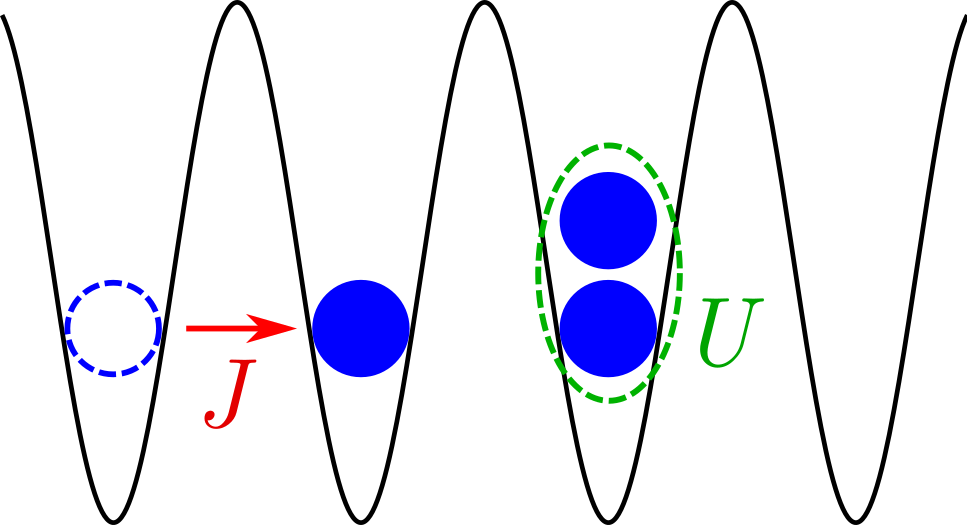
\includegraphics[width=0.5\textwidth]{Fig/Chapter2/illu_bose_hubbard.png}
    \caption[Representation of the Bose-Hubbard model]{Representation of the Bose-Hubbard model. The physics of the system are set by the tunneling coefficient $J$ and the on-site interaction energy $U$.}
    \label{fig:my_label}
\end{figure}

\begin{figure}
    \centering
    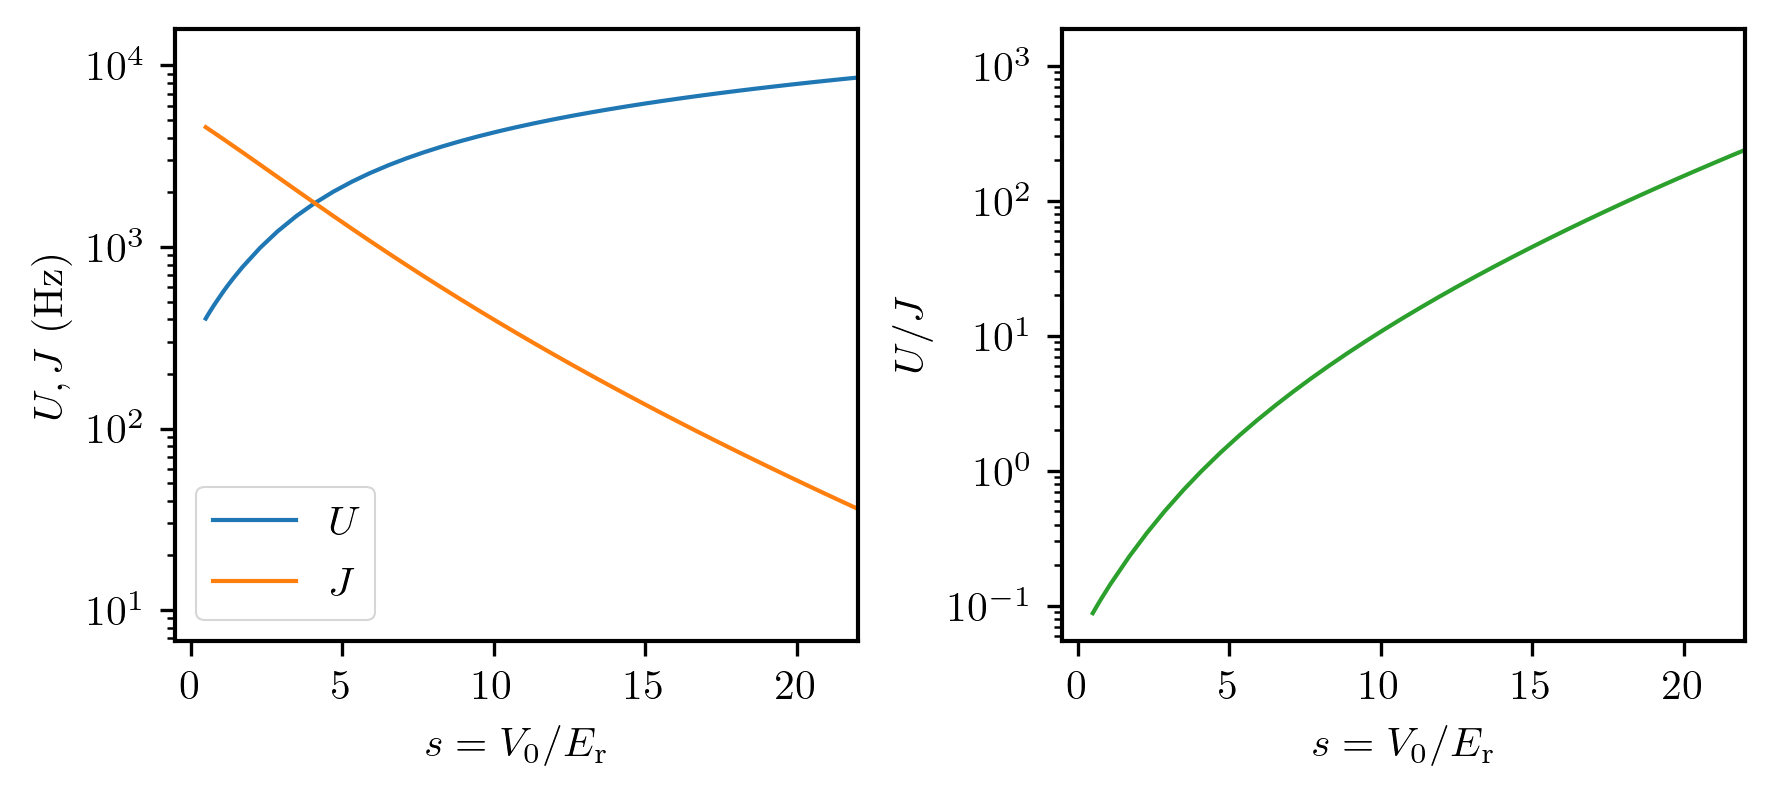
\includegraphics[width=\textwidth]{Fig/Chapter2/U_J_vs_s.png}
    \caption[Evolution of $U$, $J$ and the ratio $U/J$ as a function of the lattice depth in log-scale]{Evolution of $U$, $J$ and the ratio $U/J$ as a function of the lattice depth in log-scale from a numerical calculation with Wannier functions.}
    \label{fig:U_J_vs_s}
\end{figure}

\section{The superfluid to Mott insulator transition}

We discuss in this section the properties of the Bose-Hubbard Hamiltonian ground-state for $N$ particles spread over $M$ sites with filling $\bar{n}=N/M$. To begin, we describe the extreme cases $u \to 0$ and $u \to \infty$, which are the only cases for which the Hamiltonian can be analytically solved. 

\subsection{Extreme cases}

\subsubsection{Perfect superfluid (SF) phase $\bm{u \to 0}$}

In this case, the particles are non-interacting. In these conditions, the ground-state $\ket{\Psi_0}$ of the $N$ particles system is simply the product of the single particle ground state wave-functions, \ie the Bloch wave-functions for $q=0$ \cite{bloch2008many}:

\begin{equation}
    \ket{\Psi_0}_{\mathrm{SF}} = \frac{1}{\sqrt{N!}} (\hat{c}^{\dagger}(\bm{q}=0))^N \ket{0} = \frac{1}{\sqrt{N !}}\left(\frac{1}{\sqrt{M}} \sum_{j=1}^{M} \hat{b}_{j}^{\dagger}\right)^{N} \ket{0}
\end{equation}

\noindent The ground-state is an ideal Bose-Einstein condensate with a condensed fraction equal to 1. In the thermodynamic limit with $N \to \infty$, $M \to \infty$, it is possible to show at the price of a few lines of complex calculations \cite{gerbier_notes} that the probability to find $n_i$ atoms at a given site $i$ is:

\begin{equation}
    p\left(n_{i}\right) \approx e^{-\bar{n}} \frac{\bar{n}^{n_{i}}}{n_{i} !}
\end{equation}

\noindent We recognize the same Poissonian distribution that we obtained for a bosonic coherent state in Chapter \ref{sec:chapter_1}. We therefore write:

\begin{equation}
    \ket{\Psi_0}_{\mathrm{SF}} \approx |\Psi\rangle_{\mathrm{coh}}=\mathcal{N} e^{\sqrt{N} \hat{c}^{\dagger}(\bm{q}=0)} \ket{0} = \mathcal{N} \prod_{i} e^{\sqrt{\bar{n}} \hat{b}_{i}^{\dagger}} \ket{0} = \prod_{i} \mathcal{N}_{i} \sum_{n_{i}=0}^{\infty} \frac{\alpha_{i}^{n_{i}}}{\sqrt{n_{i} !}}\left|n_{i}\right\rangle_{i}
    \label{eq:ground-state_superfluid}
\end{equation}

\noindent with $\alpha_i=\sqrt{\bar{n}} \ \forall i \in \Z$ and the normalization factor $\mathcal{N}_{i}=e^{-\left|\alpha_{i}\right|^{2} / 2}$. We thus find that the ground state can be described as a product of local coherent states associated to the different lattice sites.

As in Chapter \ref{sec:chapter_1}, we write the first-order correlation function between two different lattice sites $i$ and $j$ to characterize the coherence properties of the ground-state:

\begin{equation}
    G^{(1)}(i,j)= \mean{\hat{b}^{\dagger}_i \hat{b}_j}
\end{equation}

\noindent In the limit $u \to 0$, $G^{(1)}(i,j)$ is easy to calculate and writes:

\begin{equation}
    G^{(1)}(i,j)= {}_{u \to 0} \bra{\Psi_0} \hat{b}^{\dagger}_i \hat{b}_j \ket{\Psi_0}_{u \to 0} = \alpha^*_i \alpha_j = \bar{n}
\end{equation}

\noindent We see that the result does not depend from the chosen lattice sites $i$ and $j$ and thus from the distance between them, indicating an infinite range coherence.


\subsubsection{Perfect Mott Insulator (MI) phase $\bm{u \to \infty}$}

In the opposite extreme limit, one can consider that the tunneling probability goes to zero $J=0$ so that each of the lattice sites are independent from one another. The Hamiltonian reduces to:

\begin{equation}
    \hat{H}_{\mathrm{BH}} = \frac{U}{2} \sum_j \hat{n}_j (\hat{n}_j -1)
\end{equation}

Because of the strong repulsive interactions, the particle localize on the lattice sites and cannot hop from site to site as $J=0$. The ground-state is then reached by distributing the particles among the different sites of the lattice so that the number of particles per site is as low as possible to minimize the interaction energy. This corresponds to putting $\bar{n}=N/M$ particles in each of the $M$ available lattice sites. For simplicity sake, we assume here that the filling is commensurate, \ie $\bar{n}$ is an integer. The ground-state then has the simple expression of a Fock state:

\begin{equation}
    \left|\Psi_{0}\right\rangle_{\mathrm{MI}}=\frac{1}{\sqrt{N !}} \prod_{j=1}^{M}\left(\hat{b}_{j}^{\dagger}\right)^{\bar{n}}|0\rangle
    \label{eq:ground-state_MI}
\end{equation}

\noindent This state is called the \textbf{Mott insulator} state \cite{fisher1989boson}. The first-order correlation function now writes

\begin{equation}
     G^{(1)}(i,j)= {}_{u \to \infty} \bra{\Psi_0} \hat{b}^{\dagger}_i \hat{b}_j \ket{\Psi_0}_{u \to \infty} = \delta_{i,j} \bar{n}
\end{equation}

\noindent and is zero when we consider any pair of different lattice sites with $i \neq j$. In the limit $J \to 0$, the system is therefore fully incoherent.



\subsection{The zero-temperature Mott phase transition}

What can then be said for intermediates values of $u=U/J$? If we start from the case $J=0$ and progressively increase $J$, it becomes possible for the atoms to hop from site to site. When an atom hops to an adjacent site, the occupancy is increased, increasing the energy by $U$. When the gain in kinetic energy $J$ is smaller than $U$, this process is unfavorable and the atoms remain localized on the lattice sites. However, when $J$ is much larger than $U$, the gain in kinetic energy outweighs the effect of the interactions and the atoms hop through the different sites of the lattice. The ground-state of the Bose-Hubbard then undergoes a phase transition as $U/J$ varies from an \textbf{insulating phase} to a \textbf{superfluid phase} with very different properties.

\begin{minipage}[t]{0.45\textwidth}
    \noindent \textbf{Superfluid phase}
    \begin{itemize}
        \item The atoms are delocalized over the entire lattice.
        \item The condensed fraction is non zero.
        \item The system shows long range coherence, \ie the phase is fixed.
        \item The on-site number of atoms is fluctuating.
        \item For low values of $u$ (far from the transition), the effect of interaction is small, so that we can use the Bogoliubov approximation (detailled later in this chapter). We find that the excitation spectrum is gapless and phonon-like at low $q$.
    \end{itemize}
\end{minipage}
\begin{minipage}[t]{0.48\textwidth}
    \noindent \textbf{Insulating phase}
    \begin{itemize}
        \item The atoms are localized on the lattice sites.
        \item The condensed fraction is zero.
        \item The system is incoherent, the phase is fluctuating.
        \item The on-site number of atoms is well defined and non fluctuating.
        \item The excitation spectrum is gapped, with the excitations consisting of particle-hole modes that can restore short-range coherence. 
    \end{itemize}
\end{minipage}

\begin{figure}
    \centering
    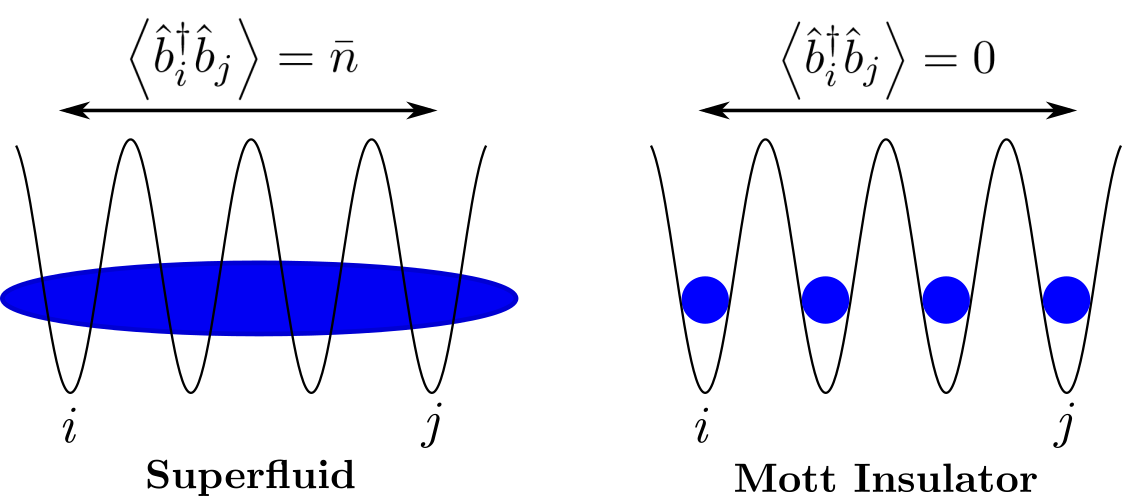
\includegraphics[width=0.9\textwidth]{Fig/Chapter2/schema_superfluid_mott.png}
    \caption[Schematic of the superfluid to Mott insulator transition]{Schematic of the superfluid to Mott insulator transition. In the superfluid phase, the atoms are delocalized and the system shows long range coherence, contrary to the Mott insulator phase where the atoms are well localized on the lattice sites, making the system incoherent.}
    \label{fig:my_label}
\end{figure}

\subsubsection{Phase diagram}

In the homogeneous case, the properties of the system thus change dramatically when $u=U/J$ crosses the \textbf{Quantum Critical Point} (QCP) $u_c$. To discuss the value of $u_c$, we slightly complexify our model where we had only considered commensurate fillings, thus fixing the chemical potential that we now set to be a free parameter. We plot on Fig.-\ref{fig:mott_lobes} the full phase diagram function of $\mu/U$, set by the filling in the Mott insulator phase $\bar{n}$ and $J/U$. As the system is homogeneous, the filling $\bar{n}$ is independent of $u$. The grey dashed lines correspond to iso-filling lines for a given value of $\bar{n}$. For commensurate fillings, the iso-filling lines cross the Mott stability lobes at the critical ratio $u_c$ that increases as the filling increases. If the filling is however incommensurate (line $n=1+\varepsilon$), we notice that the system remains in the superfluid phase as long as $J \neq 0$. This is due to the fact that a small fraction of the atoms can delocalize over the whole lattice without being blocked by the interactions $U$ as there will never be two of these particles in the same site as a consequence of the fact that the filling is incommensurate.

\begin{figure}
    \centering
    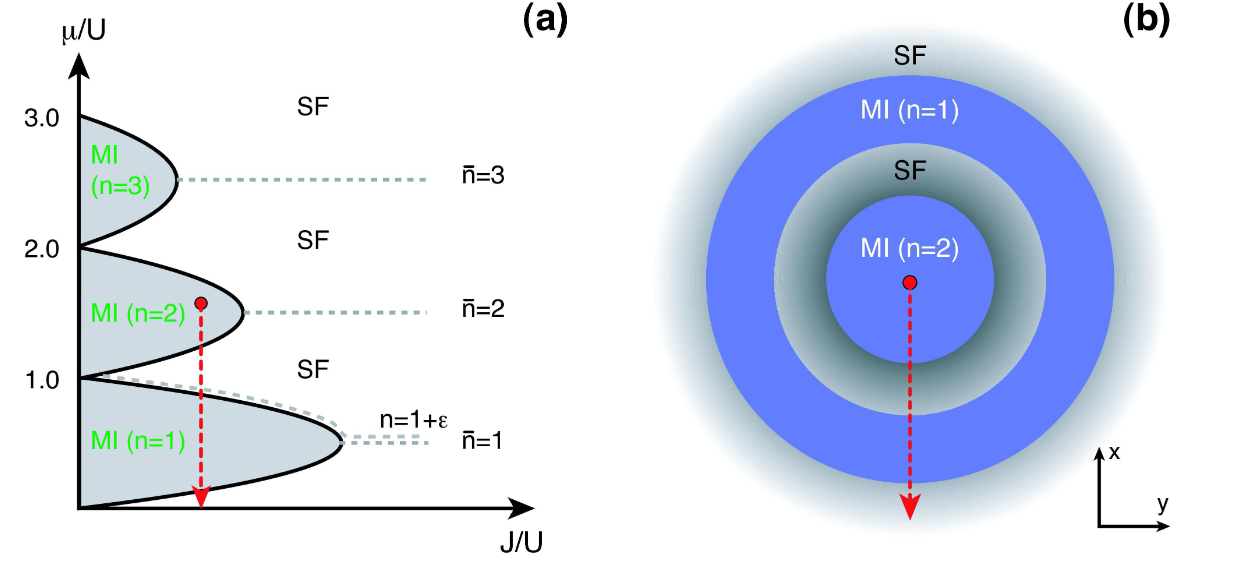
\includegraphics[width=0.9\textwidth]{Fig/Chapter2/mott_lobes.png}
    \caption[Homogeneous phase diagram as a function of $\mu/U$ and $J/U$ and wedding-cake structure for the trapped gas]{(a) Homogeneous phase diagram as a function of $\mu/U$ and $J/U$. The dashed lines are iso-filling lines. We observe a Superfluid to Mott Insulator phase transition for commensurate fillings. (b) Wedding-cake structure for the trapped gas. The red arrow illustrate how $\mu_{\rm{eff}}$ varies and the corresponding phases as the distance from the center of the trap increases. Taken from \cite{bloch2008many}.}
    \label{fig:mott_lobes}
\end{figure}

The value of $u_c$ was first calculated with mean-field theories giving out the general formula holding for any dimension $u_c=5.8z$ for $\bar{n}=1$ and $u_c=4 \bar{n} z$ for $\bar{n} \gg 1$, with $z$ being the number of nearest neighbors (6 in 3D, 4 in 2D and 2 in 1D). Later on, Quantum Monte Carlo (QMC) calculations \cite{capogrosso2007phase} simulating the 3D system for a filling $\bar{n}=1$ found $u_c=29.3(2)$, \ie slightly lower than the mean-field prediction $u_c=34.8$. For more details on this aspect, we refer the reader the the works of our team \cite{carcy_these,herce2021studying} studying the value of $u_c$ in our experiment. 



\subsection{Trapping effects}

\label{sec:ch2_trapping_effects}

In practice, the system is often not homogeneous because of the external harmonic potential $V_{\rm{ext}}(\bm{r})$ mentioned in \ref{sec:BH_model}. The properties of the trapped system can be linked to the properties of the homogeneous system by applying the Local Density Approximation\footnote{Valid as long as the trapping potential varies slowly from site to site and the system is at thermal equilibrium. This approximation may however fail at the quantum critical point \cite{pollet2012recent}.} \cite{bergkvist2004local} and replacing the chemical potential by an effective one:

\begin{equation}
    \mu_{\rm{eff}}= \mu - V_{\rm{ext}}(\bm{r})
\end{equation}

\noindent This means that the effective chemical potential, and thus the lattice filling, varies with the distance from the center of the trap. A typical situation is illustrated by the red arrow on the phase diagram of Fig.-\ref{fig:mott_lobes} where $J/U$ is small enough for Mott phases to exist and the center of the trap corresponds to a filling $\bar{n}=2$. As we get away from the center of the trap towards regions of low $\mu_{\rm{eff}}$ following the red arrow, we exit the first Mott region $\bar{n}=2$ to enter a superfluid region where the filling decreases continuously up to a second Mott region with filling $\bar{n}=1$ and finally reach a last superfluid region at the edge of the trap at vanishing values of $\mu_{\rm{eff}}$. The Mott phases are incompressible, meaning that the density remains constant even though the external trapping potential is rising, differentiating them from the superfluid region. This results in the famous ``wedding-cake'' density profile as illustrated on panel (b) of Fig.-\ref{fig:mott_lobes} and Fig.-\ref{fig:sherson}.

Actually, the external harmonic potential is quite important for experiments. If the system is homogeneous and the entropy constant, when the lattice depth is increased thus going deeper in the Mott phase, the increase of the energy gap makes it increasingly difficult for excitations to be created meaning that the temperature must increase to keep the entropy constant. In the presence of a trap however, the entropy is concentrated in the superfluid shells that can also turn to a normal gas phase, preventing the temperature of the system from increasing too much.

In the remainder of this manuscript for clarity sake, the system will be said to be in the Mott Insulator phase as long as a Mott plateau exists, \ie when $u > u_c$ where $u_c$ is the critical point for the corresponding homogeneous system.

\begin{figure}
    \centering
    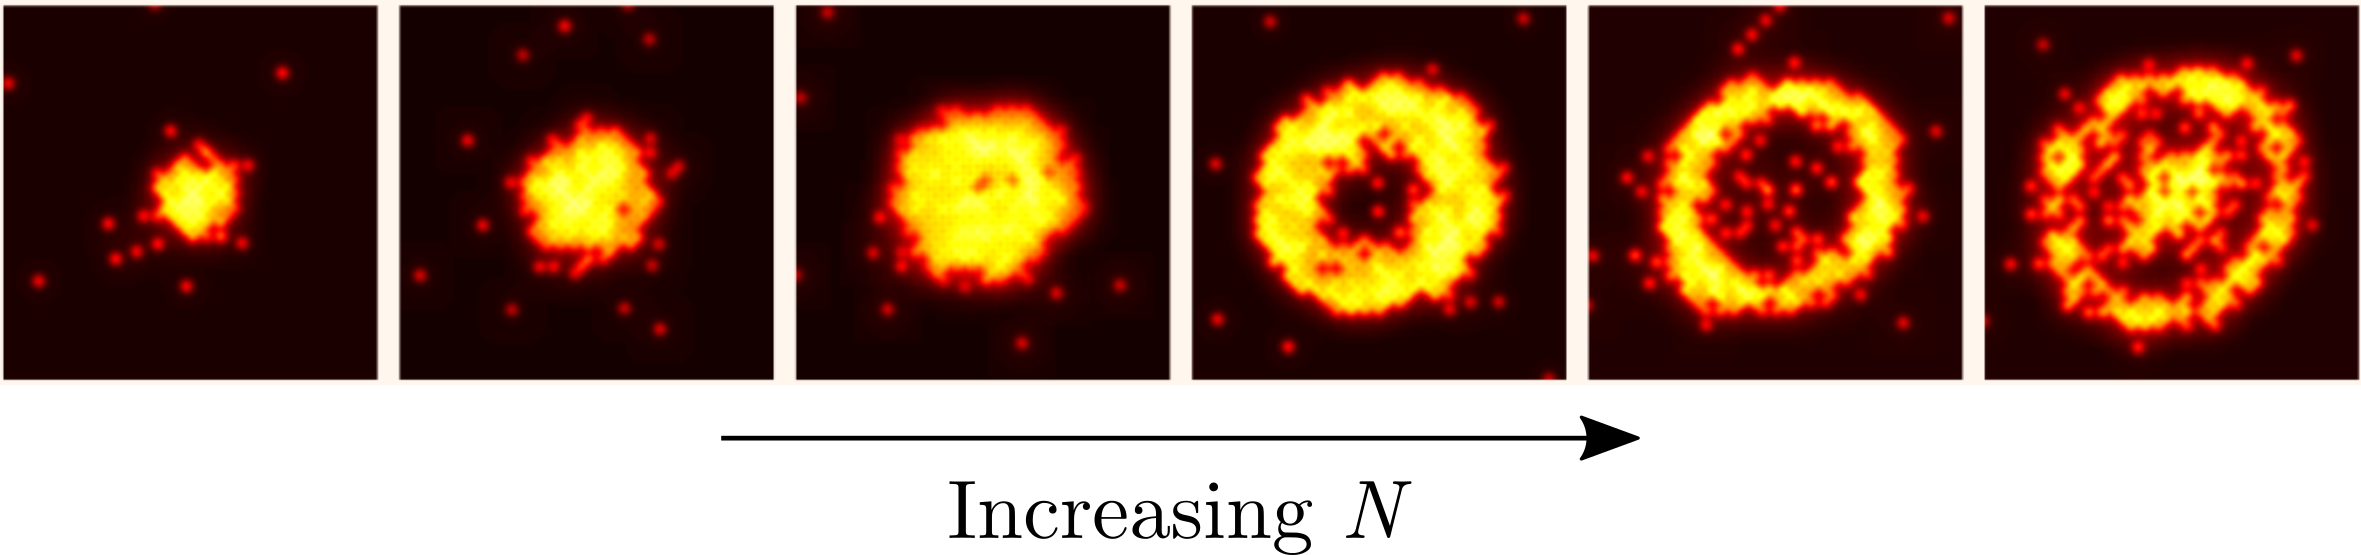
\includegraphics[width=\textwidth]{Fig/Chapter2/wedding_cake_sherson.png}
    \caption[Visualisation of the wedding cake structure with a quantum microscope experiment]{Visualisation of the wedding cake structure with a quantum microscope experiment. The imaging technique used here allows to detect the fluorescence of atoms trapped in a single site of an optical lattice, only if the number of atoms in the site is odd. We observe that as $N$ increases, the wedding cake structure appears. Taken from \cite{sherson2010single}.}
    \label{fig:sherson}
\end{figure}

\subsection{Finite temperature effects}

If we finally consider the effect of temperature, we obtain the complete phase diagram of Fig.-\ref{fig:phase_diagram} function of $T/J$ and $u$ with the apparition of an additional phase, the normal (thermal) gas. For $u \leq u_c$, the transition between the normal gas phase and the superfluid phase driven by the temperature is similar to the well-known BEC transition. This transition is induced by the thermal fluctuations and is then called classical, in opposition to the $T=0$ Mott transition which is driven by a variations of physical parameters of the Hamiltonian in the presence of quantum fluctuations and therefore is a quantum transition.

On the other hand, the Mott insulator phase also goes to the normal gas phase as the temperature increases, but with a smooth crossover. When $T$ increases, excitations are created preferably near the edges of the Mott plateaus, progressively smoothing out the sharp density profile of the Mott insulator phase. A Mott-like region survives until $T^* \sim 0.2 \ U/k_B$ \cite{gerbier2007boson} also called the ``melting temperature'' of the Mott phase.

Interestingly, the Superfluid to Mott Insulator transition subsists at low temperature. At $T=0$ and at the QCP of the transition, the ground-state undergoes a macroscopic rearrangement characterized by the apparition of critical quantum fluctuations and complex correlation patterns. Importantly, the physics of the QCP affect a signficant part of the finite temperature phase diagram as signaled by the green area on Fig.\ref{fig:phase_diagram}. In this region, some observables such as the momentum density indeed show critical behavior, \ie a power law scaling with temperature with an exponent set by the critical exponents of the QCP. While the physics of the Quantum Critical Point are a very interesting and trending topic, they fall out of the scope of this thesis and we refer the reader to the works \cite{carcy_these,frerot2019reconstructing,sachdev2011quantum} for more informations on this aspect.


\begin{figure}
    \centering
    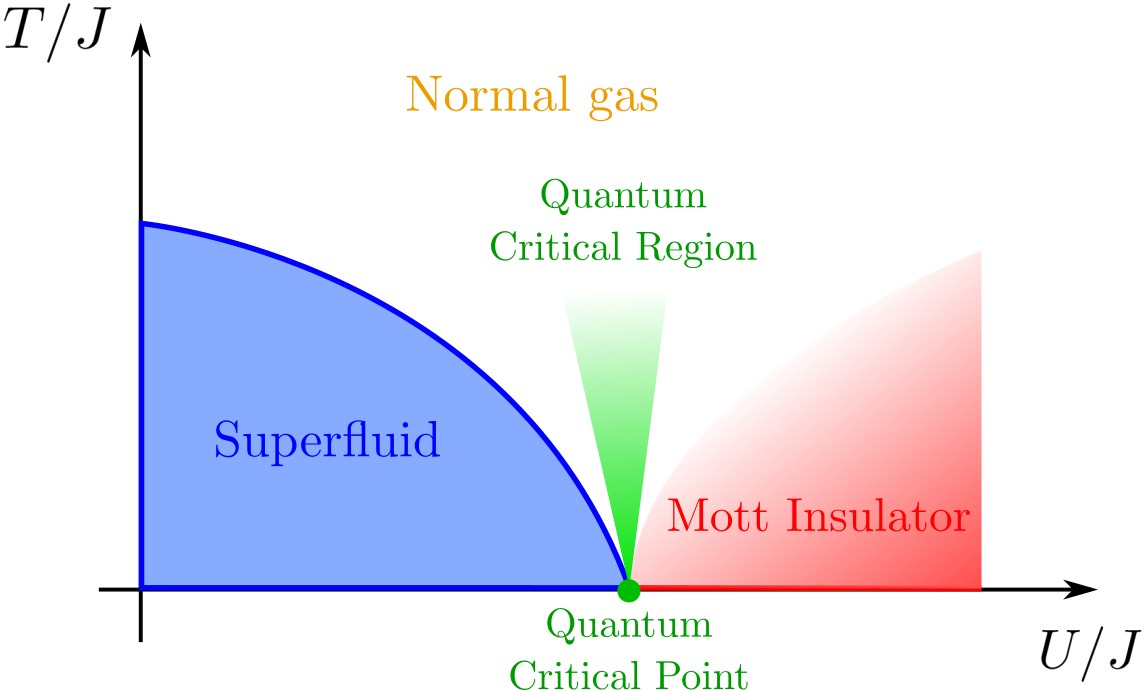
\includegraphics[width=0.78\textwidth]{Fig/Chapter2/phase_diagram.png}
    \caption[Bose-Hubbard phase diagram function of $T/J$ and $U/J$]{Bose-Hubbard phase diagram function of $T/J$ and $U/J$. We identify three phases, the Superfluid, Mott Insulator, and Normal Gas. The green area indicates the region in which critical point quantum effects could be observable in spite of the finite temperature.}
    \label{fig:phase_diagram}
\end{figure}


% The theoretical description of the Bose-Hubbard ground-state at an arbitrary value of $U/J$ is a very challenging task. It however exists a few approximate approaches from which we can obtain meaningful information as we will detail now.

\subsection{The Gutzwiller method}

\label{sec:gutzwiller}

To conclude this section, we present an approximate theoretical approach to treat the Bose-Hubbard Hamiltonian, the Gutzwiller method. This method takes its name from its author who introduced it in \cite{gutzwiller1963effect} to study strongly correlated Fermi systems. It was later adapted to characterize the ground-state of the Bose-Hubbard Hamiltonian in \cite{rokhsar1991gutzwiller}. This method is particularly useful to evaluate the density profile and therefore the size of the lattice gas with good accuracy all across the Mott transition, apart from the region close to the critical point. Although this is a ground-state, $T=0$ method that does not faithfully represent the reality of experiments, its predictions remain fairly accurate and will be quite valuable to understand the correlation signals that we will present in thesis.

The method revolves around the Gutzwiller ansatz that consists in writing the many-body ground-state as a product of on-site wave-functions $\ket{\phi_i}$:

\begin{equation}
    \ket{\Psi_G} = \prod_i^{\text{sites}} \ket{\phi_i}
\end{equation}

\noindent The on-site wave-functions are then developed on the Fock-state basis:

\begin{equation}
    \ket{\phi_i}= \sum_{n_j=0}^{\infty} f(n_j) \ket{n_j}
\end{equation}

This ansatz is motivated by the fact that it matches the exact ground-state for the extreme cases:

\begin{itemize}
    \item For $u \to 0$, the ground-state is a coherent state (see equation \ref{eq:ground-state_superfluid}) so that $f(n_j) = \mathcal{N}_{j}  (\alpha_{j}^{n_{j}})(\sqrt{n_{j} !})$ with $\alpha_j=\sqrt{\bar{n}}$ and $\mathcal{N}_{i}=e^{-\left|\alpha_{i}\right|^{2} / 2}$.
    \item For $u \to \infty$, the ground-state is already a Fock state (see equation \ref{eq:ground-state_MI}) so that $f(n_j) = \delta_{n_j,\bar{n}}$.
\end{itemize}

The Gutzwiller method is a \textbf{variational} approach, meaning that the ground-state is determined by finding the coefficients $f(n_j)$ that minimizes the free energy defined as:

\begin{equation}
    G = \mean{H_{\mathrm{BH}}}_{\ket{\Psi_G}} - \mu \mean{N}_{\ket{\Psi_G}} = -J \sum_{\langle i, j\rangle} \alpha_{i}^{*} \alpha_{j}+\sum_{j} \sum_{n_{j}=0}^{\infty}\left[\frac{U}{2} n_{j}\left(n_{j}-1\right)-\mu n_{j}\right]\left|f\left(n_{j}\right)\right|^{2}
\end{equation}

\noindent with the condition $\left\langle n_{j}\right\rangle=\sum_{n_{j}=0}^{\infty}\left|f_{j}\left(n_{j}\right)\right|^{2} n_{j}=\bar{n}$. The coefficients $f(n_j)$ can be found through numerical calculations. Interestingly, following the arguments of \ref{sec:ch2_trapping_effects}, $\mu$ can be replaced by the effective $\mu_{\rm{eff}}$ to account for the effect of the external trapping potential present in our experiment. We show on Fig.-\ref{fig:wedding_cake_gutzwiller} wedding cake density profiles for various atom numbers at $s=18$ with our experimental parameters computed with the Gutzwiller method.

\begin{figure}
    \centering
    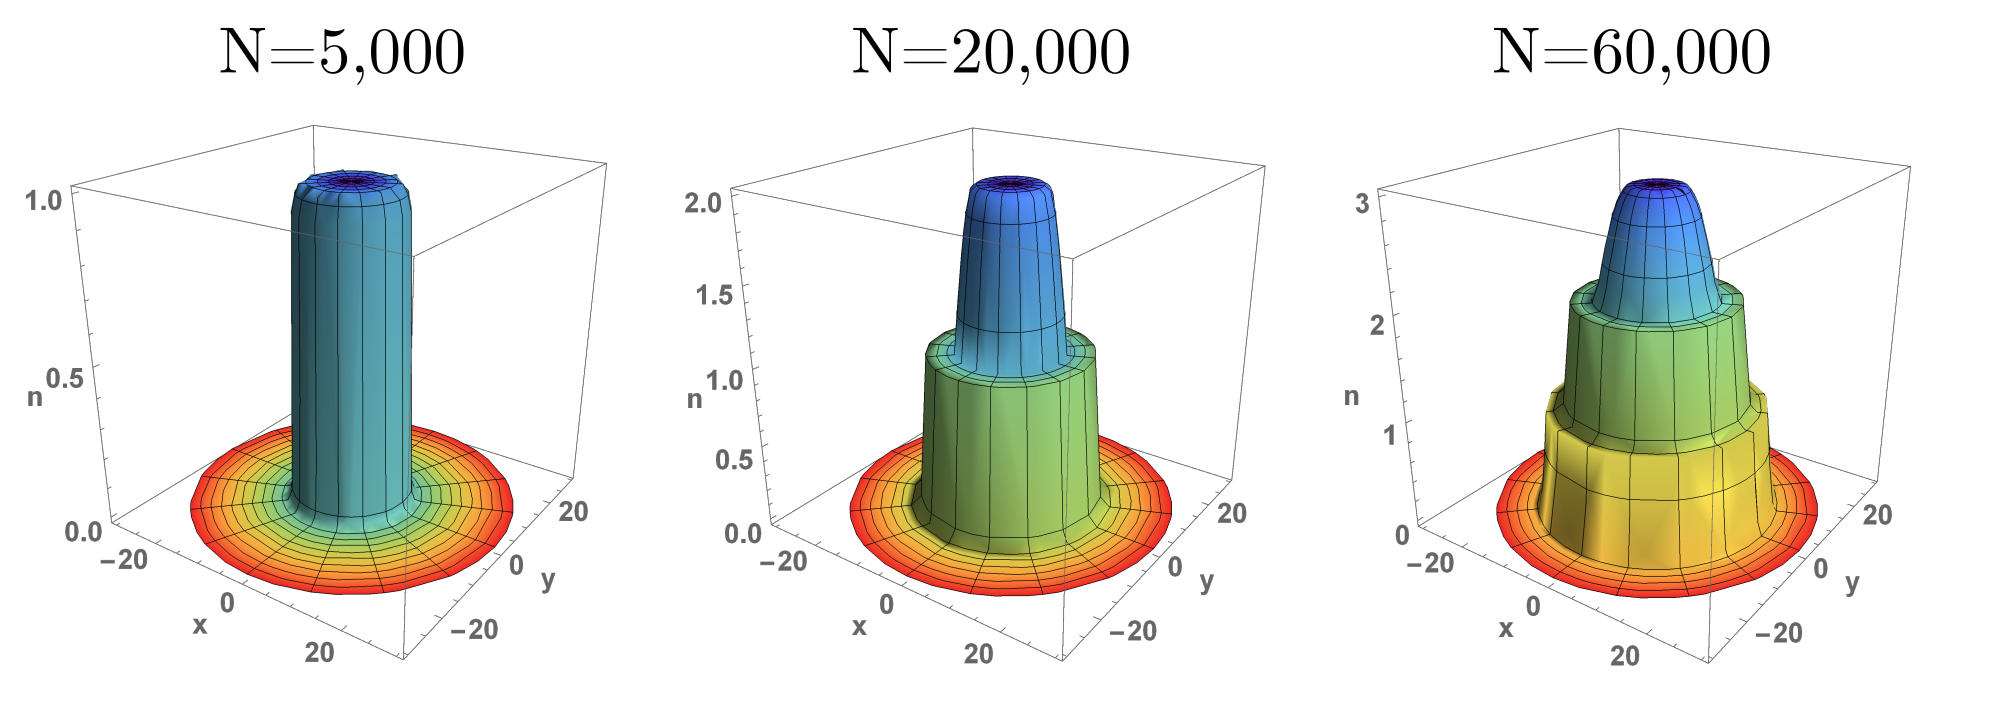
\includegraphics[width=\textwidth]{Fig/Chapter2/wedding_cake_gutzwiller.png}
    \caption[2D Gutzwiller density profiles for various atom numbers at $s=18$ with $n$ the number of atoms per site and $x$,$y$ the positions in units of lattice spacing.]{Gutzwiller density profiles for various atom numbers at $s=18$.}
    \label{fig:wedding_cake_gutzwiller}
\end{figure}


\section{Accessing the in-trap momentum distribution in a Time-Of-Flight experiment}

\label{sec:ch2_TOF}

Now that we have laid down the main elements of lattice gases physics, we need to determine the proper experimental tools to characterize the system. As developed in Chapter \ref{sec:chapter_1}, the main focus of this thesis will be on the \textbf{momentum space} correlations, requiring us to devise a technique to effectively measure the momentum distribution of a lattice gas. The most natural idea for momentum space measurements is to use the well-known and widely used \textbf{Time-Of-Flight} (TOF) technique. This technique consists in suddenly turning off the trapping potential to let the atoms fall under the effect of gravity and measure their positions $\bm{r}$ after a given TOF $t_{\rm{TOF}}$. In a very simple picture with classical and non-interacting particles, the position \bm{r} gives information about the in-trap momentum of the particle through the simple \textbf{ballistic relation}:

\begin{equation}
    \hbar \bm{k} = \frac{m \bm{r}}{t_{\rm{TOF}}}
\end{equation}

The validity of this simple relation is however far from being obvious for the quantum gases released from optical lattice. We will describe in this section the TOF dynamics of an atomic gas released from an optical lattice to identify the conditions under which a TOF measurement can be used to properly measure the in-trap momentum of the gas.

% \subsection{The momentum distribution}

% The momentum distribution of a gas of atoms on a homogeneous lattice writes \cite{gerbier2008expansion}:

% \begin{equation}
%     n(\mathbf{k}) \propto |\tilde{w}(\mathbf{k})|^{2} \sum_{i,j} e^{i \mathbf{k} \cdot (\bm{r}_i - \bm{r}_j)} G^{(1)}(i,j)
% \end{equation}

% \noindent where $\tilde{w}(\mathbf{k})$ denotes the Fourier transform of the single site Wannier function. The momentum distribution is thus strongly dependent from the lattice depth. For $U/J \to 0$, $G^{(1)}(i,j) = \bar{n}$ meaning that the momentum distribution consists of sharp peaks located at $k = j k_d$ with $j \in \Z$. In the other limit $U/J \to \infty$, $G^{(1)}(i,j) = \delta_{i,j}$ so that the momentum distribution reduces to $|\tilde{w}(\mathbf{k})|^{2}$, \ie a Gaussian-like function.

\subsection{Expansion from the lattice and Far Field regime}

We start our calculations with the simplified case for which we neglect the effects of interactions during the TOF. In this configuration, the problem is very similar to the diffraction of a light wave by a grating in optics, in which a diffraction interference pattern results from the coherent sum of the contribution of many source points associated to each of the diffraction grating holes. For the lattice gas, the source points correspond to the lattice sites associated to Wannier functions that will be able to interfere if the system is coherent. For simplicity sake, we will only consider the 1D case from which the 3D case can be easily obtained as the non-interacting Hamiltonian is separable.

At time $t=0$, right before the lattice potential is turned off, the atomic field operator writes (see \ref{eq:atom_operator_lattice})

\begin{equation}
    \hat{\Psi}(x)= \sum_{j} w_{0}(x-x_j) \hat{b}_{j} 
    \label{eq:field_operator}
\end{equation}



\noindent The expression of the Wannier functions is rather complex and very hard to handle in calculations. However, we can approximate the lattice potential near a minimum to its second-order Taylor expansion, \ie approximate it to a harmonic potential of frequency $\omega_L=2 \sqrt{s} (E_{\rm{r}}/\hbar)$ \cite{toth2008theory}. As illustrated in Fig.-\ref{fig:wannier_oh}, the Wannier function is well approximated by the Gaussian wave-function of the harmonic oscillator ground state for amplitudes $V_0 \gtrsim 10 \ \rm{E_r}$ (note however that this does not approximate tunelling well as a Gaussian function does not show the same small oscillations as the Wannier function):

\begin{figure}
    \centering
    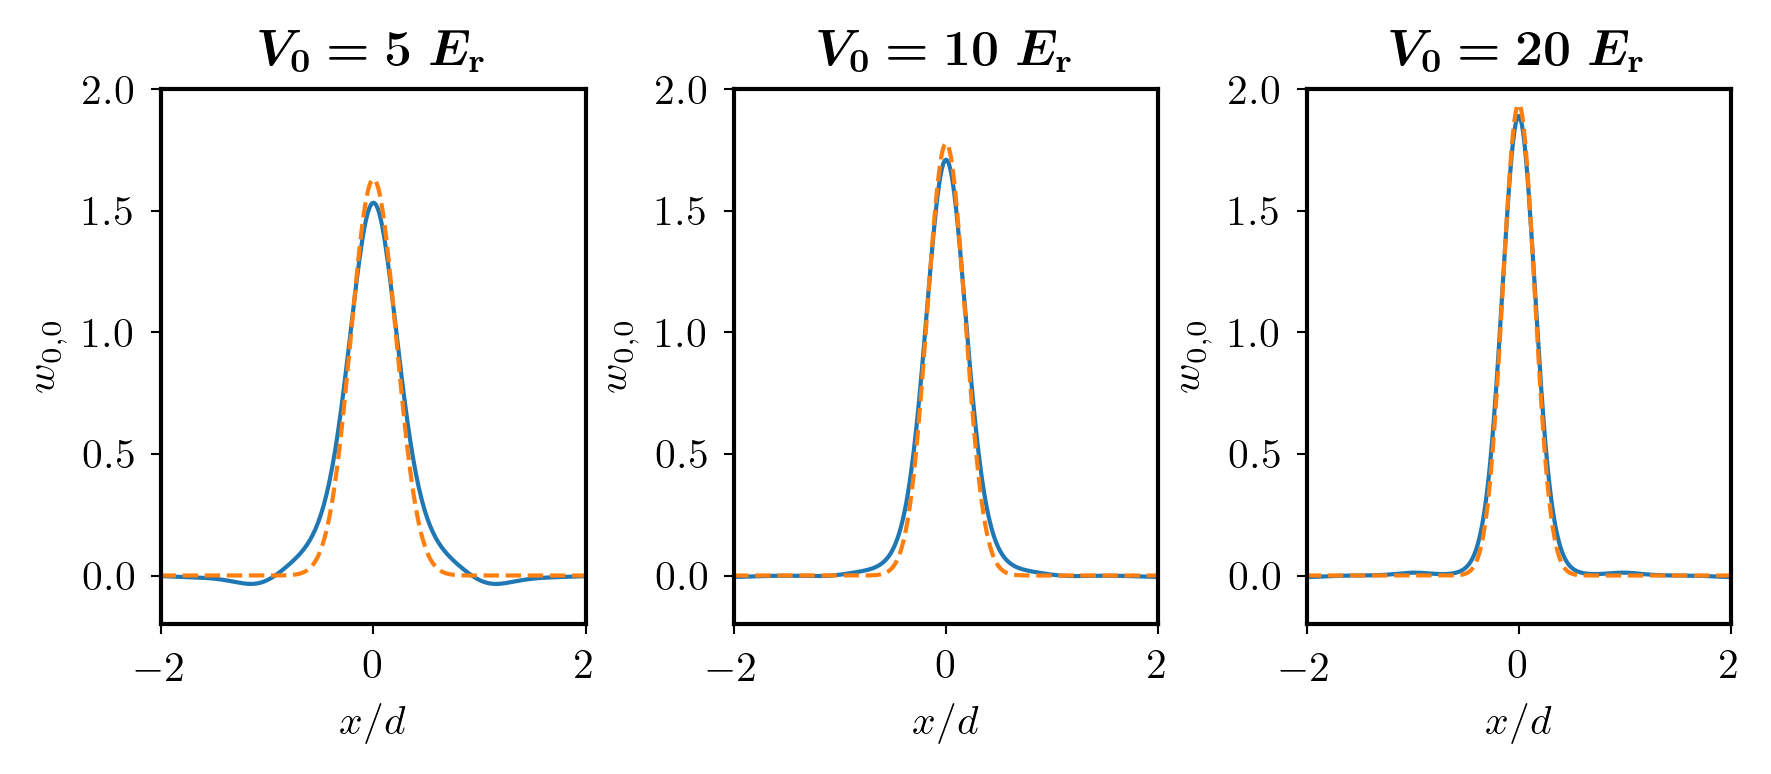
\includegraphics[width=\textwidth]{Fig/Chapter2/wannier_oh.png}
    \caption[Comparison between the Wannier functions and and the Gaussian wave-function of the harmonic oscillator of frequency $\omega_L$ for various lattice depths.]{Comparison between the Wannier functions (blue) and and the Gaussian wave-function of the harmonic oscillator of frequency $\omega_L$ (orange) for various lattice depths.}
    \label{fig:wannier_oh}
\end{figure}


\begin{equation}
    w_0(x) \simeq \frac{1}{\pi^{1 / 4} \sqrt{x_{0}}} \exp \left(\frac{-x^{2}}{2 x_{0}^{2}}\right)
\end{equation}

\noindent with $x_{0}=\sqrt{\hbar / m \omega_{L}}$.

When the lattice potential is turned off, each of the lattice sites wave-functions expand freely following the harmonic oscillator dynamics \cite{toth2008theory}:

\begin{equation}
    w\left(x-x_{j}, t\right)=\frac{1}{\pi^{1 / 4} \sqrt{W(t)}} \exp \left(-\frac{\left(x-x_{j}\right)^{2}}{2 W(t)^{2}}\right) \exp \left(-i \frac{\left(x-x_{j}\right)^{2}}{2 W(t)^{2}} \frac{h t}{m x_{0}^{2}}\right)
    \label{eq:time_dependent_wannier}
\end{equation}

\noindent with $W(t)=x_{0} \sqrt{1+\left(\hbar t / m x_{0}^{2}\right)^{2}}$ the width of the Gaussian envelope.

\subsubsection{The Far-Field regime}

In practice, as $\omega_L$ is high ($\sim 10^5-10^6 \ \rm{Hz}$), $W(t)$ increases very quickly. For instance, with $s=5$, $W(t)$ is multiplied by $\sim 600$ after $1 \ \rm{ms}$ of expansion and is thus much larger than the size of the lattice $L$. For $t>1 \ \rm{ms}$, we can make the approximation $W(t) \simeq \hbar t/m x_0$ as well as neglect the dependency on the initial site $x_j$ in the amplitude term as long as $|x| \ll W(t)$ so that we can write:

\begin{equation}
    \exp \left(-\frac{\left(x-x_{j}\right)^{2}}{2 W(t)^{2}}\right) \simeq \exp \left(-\frac{x^{2}}{2 W(t)^{2}}\right)
\end{equation}

\noindent This is equivalent to the paraxial approximation of the Fraunhofer diffraction regime in Optics.

Building up on the diffraction analogy, we would like to define an analog Fraunhofer distance where the dependency of the phase factor on the quadratic analog Fresnel term in $x_j$ can be neglected. Using $W(t) \simeq \hbar t/m x_0$, we obtain $\frac{\left(x-x_{j}\right)^{2}}{2 W(t)^{2}} \frac{h t}{m x_{0}^{2}} \simeq \frac{\left(x-x_{j}\right)^{2}}{2 x_0 W(t)}$ from which we derive the condition $\frac{x_j^2}{2 x_0 W(t)} \ll 1, \forall j$ that we rewrite \cite{gerbier2008expansion,toth2008theory}:

\begin{equation}
    t \gg t_{\rm{FF}} = \frac{mL^2}{2 \hbar}
    \label{eq:far_field}
\end{equation}

\noindent This condition defines the \textbf{Far-Field regime} after which the interference pattern is well developed, in analogy to the Fraunhofer regime of diffraction. We note the far-field regime is accessed for smaller times for lighter particles. Using one of the lightest atom, $^4 \rm{He}$, thus makes it easier to fulfill the Far-Field regime condition in the experiment. 

Combining the different approximations, we simplify \ref{eq:time_dependent_wannier} to:

\begin{equation}
    w\left(x-x_{j}, t\right)=\sqrt{\frac{m}{\hbar t}} \tilde{w_0}[Q(x,t)] \exp\left(-i \frac{\hbar Q(x,t)^{2}}{2 m} \right) \exp\left(i Q(x,t) x_{j}\right)
\end{equation}

\noindent with $Q(x,t)=\frac{m x}{\hbar t}$ and $\tilde{w_0}$ the Fourier transform of the Wannier function. 

Now that we have the general expression of $w\left(x-x_{j}, t\right)$, we generalize it to the 3D case and inject it in equation \ref{eq:field_operator} to obtain the sum of the contribution of each site:

\begin{equation}
    \hat{\Psi} (\bm{r},t) = \left(\sqrt{\frac{m}{\hbar t}} \right)^3 \tilde{w_0}[\bm{Q}(\bm{r},t)] \exp\left(-i \frac{\hbar \bm{Q}(\bm{r},t)^{2}}{2 m} \right) \sum_j e^{i \bm{Q}(\bm{r},t). \bm{r}_{j}} \hat{b}_j
\end{equation}

\noindent From this expression, we finally obtain the atomic density $\rho_{\rm{TOF}}(\bm{r},t) = \mean{\hat{\Psi}^{\dagger} (\bm{r},t) \hat{\Psi} (\bm{r},t)}$ at position $\bm{r}$ and a long TOF $t$:

\begin{equation}
    \rho_{\rm{TOF}}(\bm{r},t) = \left(\frac{m}{\hbar t} \right)^3 |\tilde{w}_0(\bm{Q}(\bm{r},t))|^2 \sum_{i,j} e^{i \bm{Q}(\bm{r},t).(\bm{r}_j - \bm{r}_{i})} \mean{\hat{b}^{\dagger}_i \hat{b}_j }
    \label{eq:rho_tof}
\end{equation}

\noindent The density $\rho_{\rm{TOF}}(\bm{r},t)$ then consists of a smooth envelope $|\tilde{w}_0(\bm{Q}(\bm{r},t))|^2$ set by the Fourier transform of the Wannier function and an interference term $\sum_{i,j} e^{i \bm{Q}(\bm{r},t).(\bm{r}_j - \bm{r}_{i})} \mean{\hat{b}^{\dagger}_i \hat{b}_j }$ that characterizes the coherence properties of the system. A numerical simulation of $\rho_{\rm{TOF}}(\bm{r},t)$ is plotted on Fig.-\ref{fig:sim_expansion} at various expansion time for $s=5$ corresponding to the superfluid phase, illustrating how the interference pattern develops in time.

\begin{figure}
    \centering
    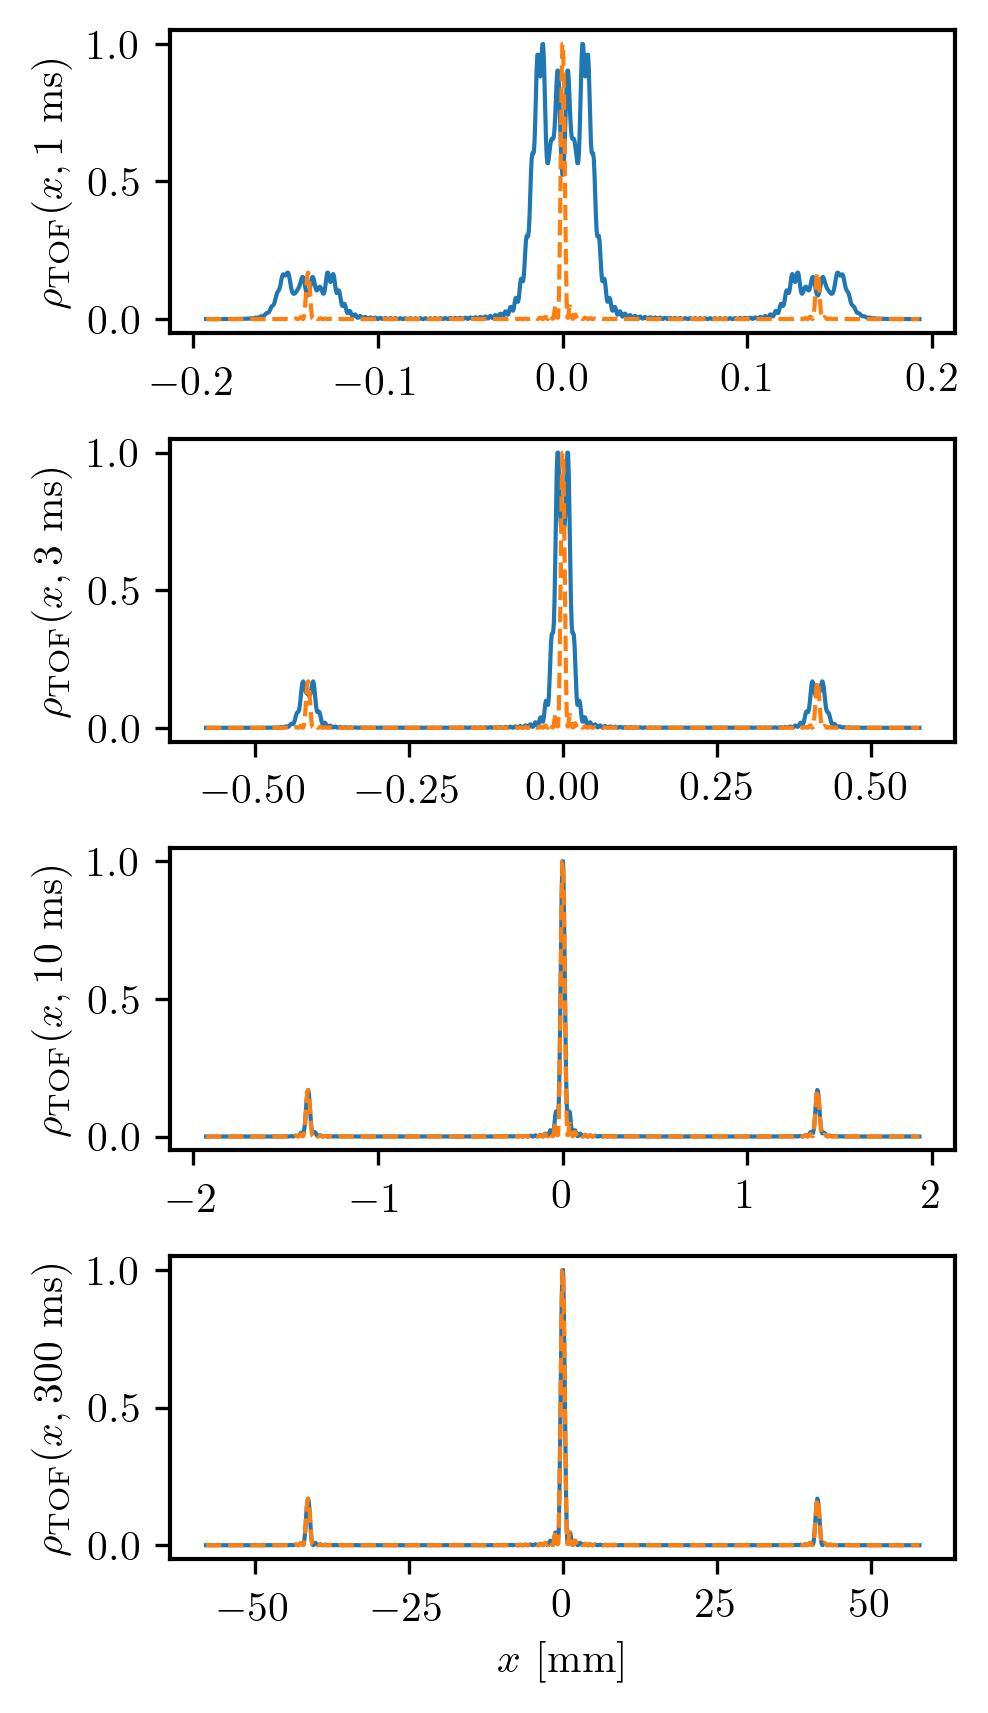
\includegraphics[width=0.7\textwidth]{Fig/Chapter2/TOF_expansion.png}
    \caption[Numerical simulation of the atomic density $\rho_{\rm{TOF}}(x,t)$ after various expansion times from a 1D lattice of 50 sites with $s=5$]{Numerical simulation of the atomic density $\rho_{\rm{TOF}}(x,t)$ after various expansion times from a 1D lattice of 50 sites with $s=5$. The orange dashed line serves as a point of comparison with the asymptotic distribution for high TOF times representing the momentum distribution.}
    \label{fig:sim_expansion}
\end{figure}

\subsubsection{Relation to the momentum distribution}

The main purpose of the TOF technique is to obtain information on the momentum distribution of the gas. To this end, we must find the relation between the measured quantity $\rho_{\rm{TOF}}(\bm{r},t)$ and the in-trap momentum distribution $\rho(\bm{k})$. To do so, we introduce the operator $\hat{a}_{\bm{k}}$ destroying a particle in mode $\bm{k}$:

\begin{equation}
    \hat{a}_{\bm{k}}=\frac{1}{\sqrt{V}} \sum_{j} e^{i \bm{k} \cdot \bm{r}_{j}} \hat{b}_{j}
\end{equation}

\noindent where $V$ is the quantization volume set to be the in-trap volume of the gas. The momentum density then writes:

\begin{equation}
    \rho(\bm{k})=\left\langle\hat{a}^{\dagger}_{\bm{k}} \hat{a}_{\bm{k}}\right\rangle=\frac{1}{V} \sum_{j, i} e^{-i \bm{k} \cdot\left(\bm{r}_{j}-\bm{r}_{i}\right)}\left\langle\hat{b}_{i}^{\dagger} \hat{b}_{j}\right\rangle
    \label{eq:momentum_distribution}
\end{equation}

\noindent If the particle are non-interacting, the ballistic relation gives $\bm{k} = m \bm{r}/\hbar t_{\rm{TOF}}$. From equation \ref{eq:rho_tof}, we obtain:

\begin{equation}
    \rho(\bm{k}) = \frac{\rho_{\rm{TOF}}(\bm{r}=\hbar t\bm{k}/m,t)}{V  \left(\frac{m}{\hbar t} \right)^3 |\tilde{w}_0(\bm{k})|^2}
\end{equation}

In conclusion, under the conditions that there are no interactions during the TOF and $t_{\rm{TOF}} \gg t_{\rm{FF}}$ to be in the far-field regime, the TOF distribution maps the in-trap momentum distribution. 

\subsubsection{Momentum distribution across the Mott transition}

As discussed previously, the momentum distribution is strongly dependent on the coherence properties of the system and in turn of the lattice depth.

\begin{itemize}
    \item In the superfluid phase $u \to 0$, the system is coherent $G^{(1)}(i,j) = \bar{n}$. From equation \ref{eq:momentum_distribution}, we get that the momentum distribution consists of sharp analog diffraction peaks located at $\bm{k} = j k_d \bm{e}_i$ with $j \in \Z$ and $\bm{e}_i$ the unitary vector in direction $i=x,y,z$. In terms of $\rho_{\rm{TOF}}(\bm{r},t)$, the amplitude of the different peaks is set by the Fourier transform of the Wannier function. 
    
    \item In the Mott insulator phase $u \to \infty$ the system is totally incoherent $G^{(1)}(i,j) = \delta_{i,j}$. The momentum distribution is then constant, meaning that $\rho_{\rm{TOF}}(\bm{r},t)$ simply reflects the Fourier transform of the Wannier function, \ie a Gaussian-like function.
    
    \item For intermediate values of $u$, the visibility of the interference pattern progressively decreases as $u$ increases. In addition, as $V_0$ increases, the Wannier function is more and more localized so that the width of its Fourier transform increases. As a result, the population of the diffracted peaks increases with the lattice depth.
\end{itemize}

The experimental quantity $\rho_{\rm{TOF}}(\bm{r},t)$ is therefore a powerful tool to characterize the phase of the system across the Mott transition. This is illustrated on Fig-\ref{fig:mott_greiner} of the first experimental observation of the Mott transition with cold atoms \cite{greiner2002quantum}, on which we can clearly see the visibility of the interference pattern decreasing with $V_0$ (note that these images are not taken deep in the far-field regime, meaning that some details of the interference pattern are not resolved).

Importantly, a characteristic of the Superfluid to Mott insulator transition is that even though the system is incoherent in the insulating phase, the coherence can be restored by ramping down the lattice depth to the superfluid phase. The standard procedure to characterize the presence of the Mott transition is then to set $V_0$ to be in the superfluid region, ramp up it up to see that the interference pattern disappear, and ramp it down to find back the interference pattern. This allows to certify that the loss of coherence is indeed an effect of the competition between $U$ and $J$ and not an experimental artifact, such as unwanted heating of the cloud. 

\begin{figure}
    \centering
    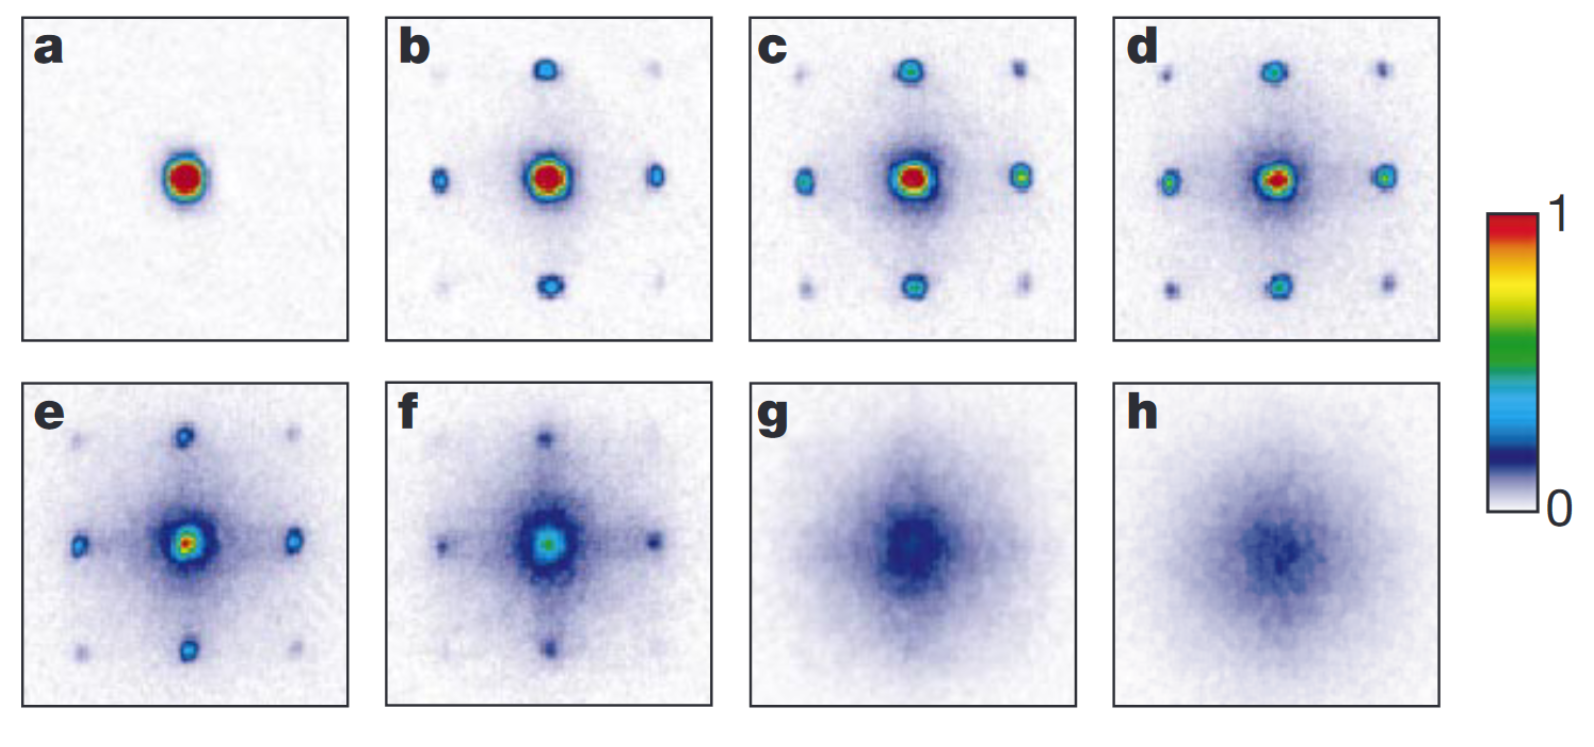
\includegraphics[width=0.9\textwidth]{Fig/Chapter2/mott_greiner.png}
    \caption[Absorption images of Rubidium atoms across the Mott transition]{Absorption images of Rubidium atoms taken $15 \ \rm{ms}$ after the atoms are released from a 3D cubic lattice. Note that the far-field regime condition is not fulfilled here. \textbf{a)} s=0. \textbf{b)} s=3. \textbf{c)} s=7. \textbf{d)} s=10. \textbf{e)} s=13. \textbf{f)} s=14. \textbf{g)} s=16. \textbf{h)} 20. Taken from \cite{greiner2002quantum}.}
    \label{fig:mott_greiner}
\end{figure}


\subsection{Mean-field interactions}

The experimental technique described in the last paragraph holds if there are no interactions between the particles during the TOF. If it were otherwise, the interactions would affect the TOF dynamics of the gas, preventing us to use the ballistic relation and to map the TOF distribution $\rho_{\rm{TOF}}(\bm{r},t)$ to the in-trap momentum $\rho(\bm{k})$. As interactions cannot be effectively turned off by means of a Feshbach resonance, experimentally inaccessible for $^4 \He$, it is crucial to determine whether interactions during the TOF can be neglected or not and under which conditions.

As mentioned in the introduction to this manuscript, describing the interactions between each of the individual particles would be impossible, even for numerical methods for which the calculation time would be prohibitive. To circumvent this issue, the problem can be simplified using the \textbf{mean-field approximation} as explained in the introduction of this manuscript.

To quantify the effect of the interactions treated at the mean-field level, we introduce the interaction energy $U_{\rm{int}} \sim gn$ with $g$ the strength of the interactions and $n$ the atomic density. To determine whether the interactions are affecting the expansion of the gas released from the lattice, $U_{\rm{int}}$ must be compared to the zero point energy of the ground-state of the approximate harmonic oscillator associated to a single lattice site, $\hbar \omega_L$. In typical experimental conditions, $U_{\rm{int}}/h \approx 10^3 \ \rm{Hz} \ll \omega_L/2 \pi \approx 10^5-10^6 \ \rm{Hz}$, meaning that the initial expansion is driven by the zero point energy of the lattice site and not the released interaction energy. In addition, after a small expansion time, the Wannier functions of the different sites overlap as their width become of the order of the lattice spacing $d$ and might then interact. However, on this time scale, the atomic density is reduced by a factor $(x_0/d)^3 \approx 10^2$ (for $s=10$), meaning that this interaction effect should also be negligible \cite{gerbier2008expansion}, provided that the initial density is not too high. This point will be discussed in further details in light of experimental data in Chapter \ref{sec:chapter_3}.

As developed in \cite{kupferschmidt2010role}, the interactions can also induce a dephasing between the different sites. As a matter of fact, the time evolution of the phase of the wave-function associated to a lattice site depends on its initial energy, and therefore of $U_{\rm{int}}$. If the lattice sites have different lattice fillings, which typically is the case in the superfluid phase where the on-site atom number fluctuations are large, the different interfering wave-functions can be dephased from one another, reducing the visibility of the interference pattern. This effect is however also negligible \cite{gerbier2008expansion,kupferschmidt2010role} in the case of our 3D lattice where $a_s \ll x_0$, provided that the filling is not too high.

\subsection{Beyond mean-field interactions}

While the mean-field approximation is efficient to obtain a first understanding on how the interactions might affect the TOF, it is inherently limited as it does not consider interaction effects between several particles. One clearly identifiable beyond mean-field effect happening during the TOF is the presence of scattering halos between the diffraction peaks \cite{greiner2001exploring}. These scattering halos signal the presence of $s$-wave collisions between the atoms of the different diffraction peaks, \ie with significantly different velocities, happening during the first moments of the TOF as they separate. This effect is analog to the scattering halos observed between two colliding condensates \cite{khakimov2016ghost,perrin2007observation,zin2006elastic}.

We have conducted a thorough experimental study of the $s$-wave two-body collisions during the TOF to determine whether they would affect our measurement of the momentum distribution \cite{tenart2020two}. This study will be detailed in Chapter \ref{sec:chapter_3}.

\section{Extension of the Bogoliubov theory to lattice gases}

So far, we have focused on the description of the lattice Hamiltonian under the scope of Wannier functions, culminating in the Bose-Hubbard Hamiltonian describing the physics of the Mott transition. We now wish to go back to the central point developed in Chapter \ref{sec:chapter_1}, namely the \kmk correlations in the quantum depletion predicted by the Bogoliubov theory of the weakly-interacting, homogeneous Bose gas. We concluded by saying that using an optical lattice would be a solution to efficiently increase the interactions as a means to reach the low temperature regime dominated by the interactions $\mu \gg \kB T$ for which we expect the pair correlation signal to be experimentally detectable. This however requires that we extend the method of the Bogoliubov theory to the case of the lattice gas to identify the condition under which the \kmk pairs should be observable.

\subsection{Effect of the lattice amplitude}

As developed in \ref{sec:bogo_approx}, the central point of the Bogoliubov approximation for the weakly-interacting homogeneous Bose gas resides in the fact that the interactions are \textbf{weak}. This means that the system can be described as a BEC from which only a \textbf{small fraction} of the atoms, the depletion, are removed by the effect of interactions.

For the lattice gas, the condensed atoms correspond to the sharp diffraction peaks of the momentum distribution, while the depleted atoms in high quasi-momentum states correspond to the diffuse background between the diffraction peaks that increases as $u$ and therefore the strength of interactions increases, as illustrated by Fig.-\ref{fig:mott_greiner}. We thus need to be in the shallow lattice regime to use the Bogoliubov approximation, \ie at low values of the lattice depth such as $u \ll u_c$. This corresponds to the superfluid phase where the condensed fraction is close to 1 and the fraction of depleted atoms is small. We will typically use $u = 5 \ll u_c \approx 30$ for the \kmk correlations experiments presented in this manuscript (the value of the fraction of depleted atoms will be discussed in Chapter \ref{sec:chapter_4}).


\subsection{Dispersion relation and effective mass}

For the remainder of this section, we will assume that we are in the shallow lattice regime so that the Bogoliubov approximation can be used. To begin, we remind the Hamiltonian for weakly interacting atoms without the lattice potential, as first introduced in Chapter \ref{sec:chapter_1}:

\begin{equation}
    \hat{H}=\sum_{\bm{k}}\frac{\hbar^2 k^2}{2m} \hat{a}^{\dagger}_{\bm{k}}  \hat{a}_{\bm{k}} +  \frac{g}{2V} \sum_{\bm{k}_1,\bm{k}_2,\bm{k}_3} \hat{a}^{\dagger}_{\bm{k_1}+\bm{k_3}} \hat{a}^{\dagger}_{\bm{k_2}-\bm{k_3}} \hat{a}_{\bm{k_1}} \hat{a}_{\bm{k_2}} 
\end{equation}

\noindent We now add the lattice potential but still neglect the external harmonic trapping potential and write the new Hamiltonian in the Bloch wave basis. In fact, we have already seen the expression of the non-interacting term in the Bloch wave basis in equation \ref{eq:H_bloch}. As we have done throughout this chapter, we consider that only the lowest energy band $n=0$ is populated. The full Hamiltonian writes \cite{dalibard2013cages}:

\begin{equation}
    \hat{H}=\sum_{\bm{q}} E_{0}(\bm{q}) \hat{c}_{\bm{q}}^{\dagger} \hat{c}_{\bm{q}}+\frac{g}{2} \sum_{\bm{q}_{1}, \bm{q}_{2}, \bm{q}_{1}^{\prime}, \bm{q}_{2}^{\prime}} C\left(\bm{q}_{1}, \bm{q}_{2}, \bm{q}_{1}^{\prime}, \bm{q}_{2}^{\prime}\right) c_{\bm{q}_{1}^{\prime}}^{\dagger} c_{\bm{q}_{2}^{\prime}}^{\dagger} c_{\bm{q}_{2}} c_{\bm{q}_{1}}
    \label{eq:lattice_bogo_hamiltonian}
\end{equation}

\noindent with $\hat{c}_{\bm{q}}$ the operator destroying a particle in the Bloch wave $\psi_{0,q}$ and 


\begin{equation}
    C\left(\bm{q}_{1}, \bm{q}_{2}, \bm{q}_{1}^{\prime}, \bm{q}_{2}^{\prime}\right)=\int_{0}^{V} \psi_{0, \bm{q}_{1}^{\prime}}^{*}(\bm{r}) \psi_{0, \bm{q}_{2}^{\prime}}^{*}(\bm{r}) \psi_{0, \bm{q}_{1}}(\bm{r}) \psi_{0, \bm{\bm{q}}_{2}}(\bm{r}) \mathrm{d} \bm{r}
\end{equation}

The non-interacting term $\sum_{\bm{q}} E_{0}(\bm{q}) \hat{c}_{\bm{q}}^{\dagger} \hat{c}_{\bm{q}}$ is quite similar to its equivalent in the homogeneous case $\sum_{\bm{k}}\frac{\hbar^2 k^2}{2m} \hat{a}^{\dagger}_{\bm{k}}  \hat{a}_{\bm{k}}$. In fact, as we can see on Fig-\ref{fig:dispersion_relation_harmonic}, the function $E_{0}(\bm{q})$ can be well approximated by a parabolic function at low values of $q$. We then rewrite $E_{0}(\bm{q})$ as:

\begin{equation}
    E_{0}(\bm{q}) \approx \frac{\hbar^2 q^2}{2 m^*}, \ \text{with } \frac{1}{m^*} = \frac{1}{\hbar^2} \frac{\mathrm{d}^2 E_0 }{\mathrm{d}q^2}
\end{equation}

\noindent where we have introduced the notion of effective mass $m^*$ defined from the curvature of the Bloch energy band, actually very useful to study the dynamics of particles in a lattice potential \cite{dalibard2013cages,kramer2002macroscopic}. Under this form, the non-interacting term of the lattice Hamiltonian is then of the exact same form as for the homogeneous Hamiltonian, the effect of the lattice being contained in the new effective mass $m^*$.

\begin{figure}
    \centering
    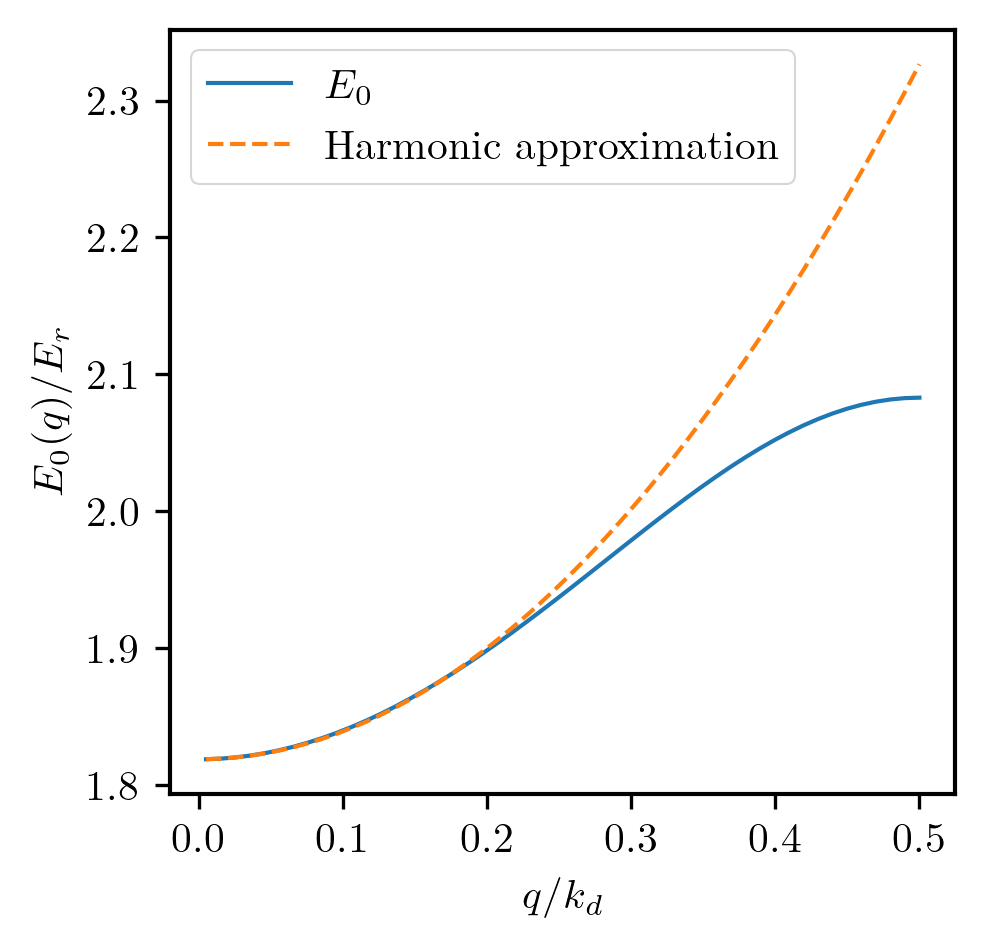
\includegraphics[width=0.5\textwidth]{Fig/Chapter2/dispersion_relation_harmonic.png}
    \caption[Harmonic approximation of the dispersion relation of the first energy band]{Harmonic approximation of the dispersion relation of the first energy band $E_0$ for $s=5$.}
    \label{fig:dispersion_relation_harmonic}
\end{figure}

In the case of non-homogeneous harmonically trapped system, the trapping frequency $\omega$ is replaced by the effective trapping frequency $\omega^*$ as well to account for the effect of the lattice. The effective frequency is defined from the effective mass by \cite{kramer2002macroscopic}:

\begin{equation}
    \omega^* = \sqrt{\frac{m}{m^*}} \omega
\end{equation}

\subsection{The rescaled interaction strength}

\label{sec:rescaled_interaction}

We turn to calculating the interaction term in equation \ref{eq:lattice_bogo_hamiltonian}. First, like in the homogeneous case, the conservation of momentum gives the relation:

\begin{equation}
    \bm{q_1} + \bm{q_2} = \bm{q}'_1 + \bm{q}'_2
\end{equation}

\noindent allowing us to reduce the sum on $\bm{q}_1,\bm{q}_2, \bm{q}'_1, \bm{q}'_2$ to a sum on three quasi-momenta $\bm{q}_1,\bm{q}_2$ and $\bm{q}_3$. Using the Bloch function form $\psi_{n,q} (x)= e^{iqx} u_{n,q} (x)$ and assuming that only the states at the bottom of the band are populated, we can finally approximate the Hamiltonian \ref{eq:lattice_bogo_hamiltonian} to \cite{dalibard2013cages}:

\begin{equation}
    \hat{H} \approx \sum_{q} \frac{\hbar^{2} q^{2}}{2 m^{*}} \hat{c}_{q}^{\dagger} \hat{c}_{q}+\frac{g^{\prime}}{2 V} \sum_{\bm{q_{1}}, \bm{q_{2}}, \bm{q_{3}}} \hat{c}^{\dagger}_{\bm{q_1}+\bm{q_3}} \hat{c}^{\dagger}_{\bm{q_2}-\bm{q_3}} \hat{c}_{\bm{q_1}} \hat{c}_{\bm{q_2}} 
\end{equation}

\noindent with $g'$ the rescaled interaction strength defined as:

\begin{equation}
    g' = g \left(d \int_0^d |w_{0,0} (x)|^4 \mathrm{d}x \right)^3
\end{equation}

\noindent that rewrites as:

\begin{equation}
    g'=g\left(\frac{\sqrt{\pi / 2} s^{1 / 4}}{\operatorname{Erf}\left[\pi s^{1 / 4} / 2\right]}\right)^{3}
\end{equation} 

\noindent As long as $V_0 > 0,$ we have $g' > g$ signaling that the lattice indeed increases the strength of the interactions. Importantly, $g'$ increases with $V_0$ as the atoms become increasingly localized in smaller region of spaces, increasing the strength of the interactions.

In conclusion, we obtain an Hamiltonian of the same form than the homogeneous case, with two notable differences:

\begin{itemize}
    \item We have replaced the mass $m$ by the effective mass $m^*$ in the dispersion relation.
    \item The interaction strength $g$ has been replaced by the rescaled and higher interaction strength $g'$.
\end{itemize}

We have then achieved the objective set at the beginning of this chapter, namely obtain a system with \kmk paired quantum depleted atoms as described by the Bogoliubov theory of the weakly-interacting Bose gas, but with increased interactions so that we should be able to reach the low temperature regime dominated by interactions $\kB T \ll \mu$ for which the \kmk correlation signal should be detectable. 

Importantly, the predictions of the Bogoliubov theory detailled in Chapter \ref{sec:chapter_1} should not be taken at face value for the much more complicated system of the inhomogeneous lattice gas. In fact, there are no clear experimental studies testing the validity of the Bogoliubov approach for this kind of system. It will then be of great interest to compare the predictions of the simple homogeneous case to the experimental data as a means to detect whether the Bogoliubov approach fails or not and under which conditions.



